\documentclass[12pt,a4paper, bold]{report}
\usepackage[utf8]{inputenc}
\usepackage{graphicx}
\usepackage{float}
\usepackage{amsmath}
\usepackage{amsthm}
\usepackage{amssymb}
\usepackage{fancyhdr}
\usepackage[a4paper,width=150mm,top=40mm,bottom=40mm,bindingoffset=6mm]{geometry}
\usepackage{indentfirst}
\setlength{\parindent}{1.5cm} % Paragraph indentation
\usepackage[toc, page]{appendix}
\usepackage[nottoc]{tocbibind}
\usepackage{tocloft} % For customizing the table of contents
\renewcommand{\cftchapdotsep}{\cftdotsep} % dots in the toc
\renewcommand{\contentsname}{\hfill\bfseries\LARGE{\uppercase{Contents}}\hfill} % centering the toc header 
\usepackage{hyperref} % Cross referencing package
\hypersetup{
    colorlinks,
    citecolor=blue,
    filecolor=black,
    linkcolor=blue,
    urlcolor=blue
}
\usepackage{setspace}
\onehalfspacing
\usepackage[style=numeric-comp,sorting=none]{biblatex}
\addbibresource{references.bib}
\fancyhead[R]{\thepage}
\cfoot{}
\pagestyle{fancy}
\graphicspath{{images/}}
\renewcommand{\familydefault}{\sfdefault}
\usepackage{physics} 
\usepackage{mathtools}
\usepackage{extarrows} 
\setlength{\parindent}{1.75em}
\usepackage{wallpaper} % For certificate superimposing 

\begin{document}
    \begin{titlepage}
    \begin{center}
        \LARGE
        \textbf{\uppercase{Development of a Python code for modeling trajectory surface hopping on \textit{ab initio} potential energy surfaces}}
        
        \vspace{1cm}
        \Large
        \textbf{\uppercase{A Thesis}}
        
        \vspace{0.4cm}
        \normalsize{\emph{submitted in partial fulfillment of the requirements \\for the award of the dual degree of}}
        
        \vspace{0.5cm}
        \large
        \textbf{Bachelor of Science - Master of Science}
        
        \vspace{0.3cm}
        \normalsize{\emph{in}}
        
        \vspace{0.3cm}
        \large
        \textbf{\uppercase{Physics}}
        
        \vspace{0.3cm}
        \normalsize{\emph{by}}
        
        \vspace{0.3cm}
        \large
        \textbf{\uppercase{Chakradhar Rangi}}
        
        \vspace{0.2cm}
        \large
        \textbf{(15200)}
        
        \vspace{0.3cm}
        
        
\includegraphics[scale=2.2]{iiserlogo.jpg}
        
        \vspace{0.5cm}
        \large
        \textbf{\uppercase{department of physics \\ Indian institute of Science education and research bhopal \\ bhopal - 462066}}
        
        \vspace{0.2cm}
        \large
        \textbf{April 2020}
        
    \end{center}
\end{titlepage}
    %-------------------- Blank page ------------------------%
    \newpage
    \thispagestyle{empty}
    \mbox{}
    \vspace*{\fill} 
    \begin{quote} 
    \centering 
    (This page is intentionally left blank)
    \end{quote}
    \vspace*{\fill}
    \pagenumbering{roman}
    \setcounter{page}{0}
%------------------ Certificate page --------------------%
    \newpage
    \fancypagestyle{certificate}{
    	\fancyhf{}
    	\cfoot{}
    	\chead{}
    	\rhead{}
    	\renewcommand{\headrulewidth}{0pt}
    }
    \thispagestyle{certificate}
    
    \ThisURCornerWallPaper{0.99}{images/letter_head_MS_Thesis.pdf}
    \vspace*{1cm}
    \begin{center}
        \LARGE{\textbf{\uppercase{Certificate}}}\label{certificate}
    \end{center}
    \vspace{2cm}
    \addcontentsline{toc}{chapter}{Certificate}
    This is to certify that \textbf{Chakradhar Rangi}, BS-MS (Dual Degree) student in Department of Physics, has completed bonafide work on the dissertation \textbf{Development of a Python code for modeling trajectory surface hopping on \textit{ab initio} potential energy surfaces} under my supervision and guidance.
    \vfill

    \noindent\textbf{April 2020 \hfill Dr. Varadharajan Srinivasan
    \\ IISER Bhopal}

    \vfill
    
    \begin{center}
        \begin{tabular}{ccc}
            \textbf{Committee Member} & \textbf{Signature} & \textbf{Date} \\
            \\
            \rule{15em}{0.4pt} & \rule{10em}{0.4pt} & \rule{6em}{0.4pt} \\
            \\
            \rule{15em}{0.4pt} & \rule{10em}{0.4pt} & \rule{6em}{0.4pt} \\
            \\
            \rule{15em}{0.4pt} & \rule{10em}{0.4pt} & \rule{6em}{0.4pt} \\
        \end{tabular}
    \end{center}
    
%------------------ Academic Integrity page --------------------%
    \newpage
    \begin{center}
        \LARGE{\textbf{\uppercase{ACADEMIC INTEGRITY AND COPYRIGHT DISCLAIMER}}}
    \end{center}
    \vspace{2cm}
    \addcontentsline{toc}{chapter}{Academic Integrity and Copyright Disclaimer}
      I hereby  declare  that  this  MS-Thesis  is  my  own  work  and,  to  the  best  of  my knowledge,  that  it  contains  no  material  previously published  or  written  by  another person,  and  no  substantial  proportions  of  material which  have  been  accepted  for  the award  of  any  other  degree  or  diploma  at  IISER  Bhopal  or  any  other  educational institution, except where due acknowledgement is made in the document. \\ \\
      I  certify  that  all  copyrighted  material  incorporated  into  this  document  is  in compliance  with  the  Indian  Copyright  (Amendment)  Act  (2012)  and  that  I  have received  written  permission  from  the  copyright  owners  for  my  use  of  their  work, which  is  beyond  the  scope  of  that  law.  I  agree  to  indemnify  and  saveguard  IISER Bhopal from any claims that may arise from any copyright violation. 
      
      \vfill 
      
      \noindent\textbf{April 2020 \hfill Chakradhar Rangi
    \\ IISER Bhopal}
    
%------------------ Acknowledgment --------------------%
    \newpage
    \begin{center}
        \LARGE{\textbf{\uppercase{Acknowledgement}}}
    \end{center}
    \vspace{1cm}
    \addcontentsline{toc}{chapter}{Acknowledgement}
    My MS thesis is an outcome of the contributions played by a lot of people directly and indirectly. Foremost, I would like to express my deepest gratitude to my Supervisor, Dr. Varadharajan Srinivasan, for his continuous guidance, enthusiastic encouragement, and insightful critique of this work. I am grateful for his willingness to dedicate his time to the extended discussion sessions that instilled confidence and helped me tackle tough roads of this journey. \\ \\
    My journey at IISER Bhopal comes to an end with the submission of this thesis and I would like to thank all my teachers of the Physics department who contributed to my learning and understanding of concepts in Physics. \\ \\ 
    I sincerely thank Satyajit Mandal and the entire members of the Ab Initio Theory group at IISER Bhopal for their invaluable insights and much needed help during the inception. I also thank IISER Bhopal for providing the computational resources which were essential for the completion of this work. \\ \\
    Being part of the cricketing fraternity at IISER Bhopal has helped reshape my character. Through this journey I have learnt the importance of being passionate, competitive and team work. I sincerely thank Mr. Mukesh Kanaujia and rest of the fraternity for being part of this memorable journey. A special mention goes to Mr. Sudarshan Sharma for luring me into the cricketing world at IISER Bhopal and always helping me in difficult times.  \\ \\
    No journey is complete without friends. I would like to thank Abhijeet, Akhil, Anirudha, Anoop, Aritra, Arundhati, Ashutosh, Bikram, Bhupendra, Bhushan, Hricha, Keshav, Madhur, Mahesh, Manav, Nihal, Nikhila, Raghuveer, Sagar, Shreyas, Sonal, Soumya, Sreshta, Subhaprad, Sushmita, Tejas, Viswajeet, Yadunandan and all those whom I have missed in this list for their valuable support and discussions that provided me a new perspective to this life. And lastly I would like to thank my parents who are, and will always be people whom I love, respect and revere. They have always encouraged me and supported me throughout my life.
    \vfill 
    \noindent\textbf{\hfill Chakradhar Rangi}
    
%------------------ Abstract --------------------%
    \newpage
    \begin{center}
        \LARGE{\textbf{\uppercase{Abstract}}}
    \end{center}
    \vspace{2cm}
    \addcontentsline{toc}{chapter}{Abstract}
    We aim at developing and implementing a Python-based trajectory surface hopping layer to a localized basis electronic structure code (NWChem). Non-adiabatic dynamics is crucial for simulating excited-state phenomena such as photo-induced charge transfer, photo-chemical reactions, etc. For large-scale systems it is important to speed up the electronic structure calculation which can be achieved by using localized basis codes. NWChem is a highly parallel gaussian basis code which, however, does not currently have a built-in functionality for non-adiabatic dynamics. By creating our own layer for non-adiabatic dynamics and interfacing it with NWChem we plan to have a highly efficient code for simulating excited-state dynamics in large-scale systems.
    
    
%------------------ List of Figures --------------------%
    \newpage
    \begin{center}
        \listoffigures
    \end{center}
    \vspace{2cm}
    
%------------------ Table of contents ------------------%
    \newpage
    \tableofcontents
    \newpage
    \thispagestyle{empty}
    \mbox{}
    \vspace*{\fill} 
    \begin{quote} 
    \centering 
    (This page is intentionally left blank)
    \end{quote}
    \vspace*{\fill}
    
%----------------- Quote -----------------------%

\newpage
\thispagestyle{empty}
\mbox{}
\vspace*{\fill} 
\begin{quote} 
\centering 
"We need science education to produce scientists, but we need it equally to create literacy in the public. Man has a fundamental urge to comprehend the world about him, and science gives today the only world picture which we can consider as valid. It gives an understanding of the atom and of the whole universe, or the peculiar properties of the chemical substances and of the manner in which genes duplicate in biology. An educated layman can, of course, not contribute to science, but can enjoy and participate in many scientific discoveries which as constantly made. Such participation was quite common in 19th century, but has unhappily declined. Literacy in science will enrich a person's life."

- Hans A Bethe
\end{quote}
\vspace*{\fill}
\newpage
\thispagestyle{empty}
\mbox{}
\vspace*{\fill} 
    \begin{quote} 
    \centering 
    (This page is intentionally left blank)
    \end{quote}
\vspace*{\fill}
\pagenumbering{arabic}
\setcounter{page}{0}
    
    \chapter{Introduction}
    \section{Motivation}

The Born-Oppenheimer(adiabatic) approximation\cite{Born_Oppen} is a widely used concept in the description of quantum states of a molecule and is motivated by the fact that the nuclei are much more massive than electrons. This apparent difference in mass leads to a difference in energy scales and consequently the time scale for nuclear evolution is much larger compared to  electrons. This  aids to decouples the molecular Hamiltonian into electronic and  nuclear degrees of freedom. The electronic Hamiltonian is solved by parametrically varying nuclear positions and the resulting  eigenenergies, which is now a function of nuclear positions,are  termed as the Potential energy surfaces(PES). The adiabatic  theorem then allows us to realise the dynamics of nuclei, by propagating them on a single PES. Usage of single PES for nuclear propagation is termed as adiabatic dynamics. \\ \\
However, there are wide system of interest such as photo-induced charge transfer, photo-chemistry, photo-stability of the genetic code, quantum information processing with atomic and molecular qubits, etc.,\cite{app_1,app_2,app_3} which cannot be adequately described within this approximation and non-adiabatic dynamics are crucial to capture such phenomenon. There are wide variety of semi-classical methods available to incorporate such non-adiabatic effects.\cite{tully_discussion} The abundance of such treatments thrives  on conceptual simplicity and computational efficiency. The trajectory surface hopping(TSH) scheme is one such approach in which nuclei are propagated using classical laws and electrons are treated in quantum mechanical fashion.\cite{tully_1,tsh_barbatti,wang_TSH,TSH_review} It uses molecular dynamics(MD) simulations to propagate nuclei adiabatically on PES subject to switching the surface according to a stochastic algorithm. \\ \\
The TSH scheme has been successfully extended to many-body systems by combining it with many theoretical tools such as Density Functional Theory, Time-dependent Density Functional Theory(TDDFT) and Linear response-TDDFT.\cite{dft_tsh,tddft_tsh,Tavernelli} The algorithm for TSH has been implemented in various packages such as NEWTON-X(integrates with Turbomole,Gaussian).\cite{newton-x} Unfortunately, calculations in the above implementations suffer in handling large molecules since the code is only parallel over different processors of the same node. This demands in developing a highly parallel code distributed over different nodes and use of localised basis to speed up the calculations. The above codes are also not open source. The open source movement is the reason that technology has developed at such a breathtaking pace for the past few decades. It also welcomes collaboration which is an important aspect of scientific community to solve crucial problems. NWChem aims to provide its users with computational chemistry tools that are scalable both in their ability to treat large scientific computational chemistry problems efficiently, and in their use of available parallel computing resources from high-performance parallel supercomputers to conventional workstation clusters.\cite{nwchem} This paves a way to tackle the computational inefficiency in large-scale and the code is distributed as open-source under the terms of the Educational Community License version 2.0 (ECL 2.0). Thus, our interest lies to build an efficient TSH Python layer on top of NWChem to gain a code which is readable, modular, efficient and open source. 

\section{Quantum Adiabatic Theorem}

The dynamics of a quantum system with Hamiltonian $\mathcal{H}(t)$ is governed by the Scr{\"o}dinger equation,
    \begin{equation}\label{td_schrodinger_eqn}
        i\hbar\frac{\partial}{\partial t}\ket{\psi(t)} = \mathcal{\hat{H}}(t)\ket{\psi(t)}
    \end{equation}
The evolution is straightforward if the Hamiltonian is time independent: 
$\ket{\psi(t)} = \text{exp}(-i\mathcal{H}t)\ket{\psi(0)}$ i.e., the system remains in the initial physical state up to a dynamical phase. If the Hamiltonian explicitly depends on time, the dynamics can be fairly complicated. However, if the Hamiltonian varies slowly with time, the Quantum Adiabatic Theorem provides us the evolution.\cite{griffiths_schroeter_2018} It states: \par \vspace{0.4cm} \textit{A physical system remains in its instantaneous eigenstate if a given perturbation is acting on it slowly enough and if there is a gap between the eigenvalue and the rest of the Hamiltonian's spectrum.} \vspace{0.4cm} \\ 
Simply stated, the system remains in the eigenstate which it is presently in given the conditions above are satisfied. We lay out the proof in a rough manner. The instantaneous eigenstate equation is defined as follows:
    \begin{equation}
        \mathcal{\hat{H}}(t)\ket{\varphi_n(t)} = E_n(t)\ket{\varphi_n(t)}
    \end{equation}
This equation is solved parametrically varying '$t$' generating an eigenvalue trajectories in the parameter space. The instantaneous eigenstates generated in this way are used to solve \eqref{td_schrodinger_eqn}\footnote{Please note that these eigenstates are in no way exact solutions of the time-dependent Schrodinger equation} by constructing the ansatz given below:
    \begin{equation}
        \ket{\psi(t)} = \sum_n C_n(t) \ket{\varphi_n(t)}
    \end{equation}
Substituting in \eqref{td_schrodinger_eqn}, solving for coefficients $C_k(t)$, we get
    \begin{equation}
         i\hbar\Dot{C_k} = \left(E_k -i\hbar\bra{\varphi_k}\ket{\Dot{\varphi _k}}\right)C_k -i\hbar\sum_{n\neq k}\frac{(\Dot{H})_{nk}}{E_k-E_n}C_n
    \end{equation}
We observe that the adiabatic theorem holds when the second term on the right hand side is neglected. Intuitively, this term can be neglected, whenever the Hamiltonian is varying slowly and the eigenvalues are not close to degenerate. Thus, by neglecting the last term on the right, the system evolves on the same instantaneous eigenstate. 
    \begin{equation}
         i\hbar\Dot{C_k} \approx \left(E_k -i\hbar\bra{\varphi_k}\ket{\Dot{\varphi _k}}\right)C_k
    \end{equation}
The above approximation constitutes the quantum adiabatic theorem. 
\section{Born-Oppenheimer Approximation}

For molecules, we can write the Hamiltonian in the atomic units as:
\begin{equation}\label{molecular_Hamiltonian}
    \mathcal{\hat{H}}_{\text{mol}} = \sum_{\alpha}^{N_n}\frac{-1}{2M_\alpha}\nabla^2_\alpha + \sum_i^{N_e}\frac{-1}{2m_i}\nabla_i^2 - \sum_i^{N_e}\sum_\alpha^{N_n}\frac{Z_\alpha}{|\mathbf{R_\alpha}-\mathbf{r_i}|} + \sum_{i<j}\frac{1}{|\mathbf{r_i}-\mathbf{r_j}|} + \sum_{\alpha<\beta}\frac{Z_\alpha Z_\beta}{|\mathbf{R}_\alpha-\mathbf{R}_\beta|}
\end{equation}
which represents nuclear \& electronic kinetic energy, electrostatic interaction between nuclei-electron, electron-electron \& nuclei-nuclei repulsion. The time-dependent Schr{\"o}dinger equation is given by
\begin{equation}\label{td_mole_schrodinger}
    i\hbar\frac{\partial}{\partial t}\Psi(\mathbf{r},\mathbf{R},t) = \mathcal{\hat{H}}_{\text{mol}}\Psi(\mathbf{r},\mathbf{R},t) \equiv \left(\sum_\alpha^{N_n}\frac{-\hbar^2}{2M_\alpha}\nabla_\alpha^2 + \mathcal{\hat{H}}_{\text{el}}\right)\Psi(\mathbf{r},\mathbf{R},t)
\end{equation}
One of the aspects of the Hamiltonian in \eqref{molecular_Hamiltonian} is the coupling between the nuclear and electronic degrees of freedom due to the nuclear-electron attraction term making it difficult to solve \eqref{td_schrodinger_eqn}. 

A key idea is to note that the nuclei are massive than electrons leading to a huge difference in the energy scale between these two degrees of freedom. By employing the quantum adiabatic theorem\cite{griffiths_schroeter_2018,adi_appx_zwiebach}, we can effectively reduce the complexity of the problem as follows: 
\begin{itemize}
    \item The electronic Schrodinger equation 
    \begin{equation}
         \mathcal{\hat{H}}_{\text{el}}\psi_k(\mathbf{r};\mathbf{R}) = E^{\text{el}}_k(\mathbf{R})\psi_k(\mathbf{r};\mathbf{R})
    \end{equation}
    is solved by parametrically varying the nuclear configurations\footnote{$\mathbf{R}$ is no longer an operator. It is just a parameter now}. 
    \item The instantaneous eigenvalue $E^{\text{el}}_k(\mathbf{R})$ becomes the potential surface for the nuclei to move on
    \begin{equation}
        \left(\sum_{\alpha}^{N_n}\frac{-1}{2M_\alpha}\nabla^2_\alpha + E^{\text{el}}_k(\mathbf{R}) \right)\Omega_I(\mathbf{R}) = E_I\Omega_I(\mathbf{R})
    \end{equation}
\end{itemize}
The above approximation which is motivated by the physical fact that the nuclei are massive than electrons is termed as the Born-Oppenheimer approximation(BO). It is one of the fundamental approximations in chemistry. 

\section{Failure of Born-Oppenheimer Approximation: \\Non-adiabatic Dynamics}

The Born-Oppenheimer approximation, although one of the fundamental approximations, has its limitations. There are wide variety of chemical and physical processes such photo-induced charge transfer, internal conversion, inter-system crossing, etc., where this adiabatic approximation breaks down and non-adiabatic dynamics is crucial to understand such phenomena. Primarily, it is important to understand the reasons for this breakdown. More precisely, we want to figure out the conditions that lead to the failure of the BO approximation. \\ \\
The BO approximation is essentially an application of the Quantum adiabatic theorem. Let us inspect the error term that we ignored while proving the theorem: 
\begin{equation}\label{error_QAT}
    \text{error} = -i\hbar\sum_{n\neq k}\frac{(\Dot{H})_{nk}}{E_k-E_n}C_n
\end{equation}
It is evident from the expression above that the:
\begin{itemize}
    \item error blows up whenever the energy levels are degenerate i.e., the energy surfaces cross each other. This is a well known phenomena in chemistry as the conical intersection. 
    \item error is very significant if the matrix element of the rate of change of the Hamiltonian with respect to the parameter is larger than the energy difference between the states in consideration i.e., $|(\Dot{H})_{nk}| \gtrsim |E_n - E_k|$. 
\end{itemize}
Let us rephrase the last point in a more suitable manner for our purposes. In case of molecular systems(assuming the BO approximation), the parameters which are varying slow are the nuclear coordinates $\mathbf{R}\equiv (\mathbf{R_1},\mathbf{R_2},...,\mathbf{R_n})$. As pointed out before, $\mathbf{R}$ is no longer an operator and it implicitly carries the temporal dependence $\mathbf{R}(t) = (\mathbf{R_1}(t),\mathbf{R_2}(t),...,\mathbf{R_n}(t))$. Thus, \eqref{error_QAT} becomes
\begin{align}
    \text{error} \propto \frac{(\Dot{H})_{nk}}{E_n-E_k} &= \frac{\mel**{n}{d\mathcal{\hat{H}}_{mol}(\mathbf{R}(t))/{dt}}{k}}{E_k - E_n} \\
    &= \frac{\mel**{n}{\nabla_{\mathbf{R}}\mathcal{\hat{H}}_{mol}\cdot \dot{\mathbf{R}}}{k}}{E_k - E_n} \\
    &= \frac{\mel**{n}{\nabla_{\mathbf{R}}\mathcal{\hat{H}}_{mol}}{k}}{E_k - E_n}\cdot \dot{\mathbf{R}} \\ 
    &= \mathbf{d}_{nk} \cdot \dot{\mathbf{R}}
\end{align}
where 
\begin{equation}\label{NAC}
    \mathbf{d}_{nk} = \frac{\mel**{n}{\nabla_{\mathbf{R}}\mathcal{\hat{H}}_{mol}}{k}}{E_k - E_n} = \mel**{n}{\nabla_{\mathbf{R}}}{k}
\end{equation}
is the non-adiabatic coupling vector and it gives us a quantitative measure of the error in the BO approximation. It will help us to characterize non-adiabatic processes. 
    
    \chapter{Theoretical Overview}
    \section{Trajectory Surface Hopping}
Trajectory surface hopping is a mixed quantum-classical approach to simulate the non-adiabatic dynamics.\cite{tully_1,dephasing_2} Its wide popularity is attributed to its intuitive conceptual background and high computational efficiency in contrast to full quantum mechanical propagation. It is based on the hypothesis that the dynamics of nuclear wave-packet through a PES branching region can be approximated by an ensemble of independent classical trajectories distributed stochastically amongst the branching surfaces.
    In a broad sense, the classical  trajectories  corresponding  to  the  nuclei  are  propagated  along  the  potential  energy surfaces in an adiabatic fashion using MD simulations subject to change the electronic state according to a stochastic  algorithm. The molecular dynamics simulations are employed due to its ability to treat nuclei in full dimensionality. The  statistical  character of the wave packet is approximated by statistical ensemble of independent trajectories.

\subsection{The Method}
    The molecular Hamiltonian which governs the electronic and nuclear motion is given by
    \begin{equation}
        \Hat{\mathcal{H}}_{\text{mol}} = \hat{\mathcal{T}}_{\mathbf{R}} + \Hat{\mathcal{H}}_{\text{el}}(\mathbf{r},\mathbf{R})
    \end{equation}
    where $\Hat{\mathcal{H}}_{\text{el}}(\mathbf{r},\mathbf{R})$ is the electronic Hamiltonian and $\hat{\mathcal{T}}_{\mathbf{R}}$ denotes the nuclear kinetic energy operator. Here, $\mathbf{r}$ and $\mathbf{R}$ denote electronic and atomic coordinates respectively. The nuclear coordinate $\mathbf{R} \equiv \mathbf{R}(t)$ is what we will be referring to as the classical trajectory. We now choose any orthonormal set of electronic basis functions $\varphi_j(\mathbf{r},\mathbf{R})$  which parametrically depends on the nuclear coordinates. For definiteness here, we construct the ansatz for the electronic wavefunction using adiabatic states $\{\psi_j\}$,
    \begin{equation}\label{ansatz}
        \Psi^\alpha(\mathbf{r},\mathbf{R},t) = \sum_j c^\alpha_j(t) \psi_j(\mathbf{r};\mathbf{R})
    \end{equation}
    The superscript $\alpha$ denotes the trajectory dependence and adiabatic states are eigenstates of the electronic Hamiltonian:
    \begin{equation}
        \hat{\mathcal{H}}_{\text{el}}\psi_j(\mathbf{r};\mathbf{R}) = E_j(\mathbf{R})\psi_j(\mathbf{r};\mathbf{R})
    \end{equation}
    The time-dependent electronic Schr{\"o}dinger equation is given by
    \begin{equation}\label{TDSE}
        i\hbar\frac{\partial}{\partial t}\Psi^\alpha(\mathbf{r},\mathbf{R},t) = \Hat{\mathcal{H}}_{\text{el}}(\mathbf{r},\mathbf{R})\Psi^\alpha(\mathbf{r},\mathbf{R},t) 
    \end{equation}
     Inserting the ansatz \eqref{ansatz} into \eqref{TDSE}, multiplying by $\psi_k$ and integrating with respect to $\mathbf{r}$ gives
     \begin{equation}\label{cdot}
         i\hbar \Dot{c}_k^\alpha(t) = c_k^\alpha(t)E_k(\mathbf{R}) - i\hbar\sum_j c_j^\alpha(t)\Dot{\mathbf{R}}^\alpha\cdot\mathbf{d}^\alpha_{kj} 
     \end{equation}
     where the non-adiabatic coupling vector $\mathbf{d}_{kj}$ is given by
     \begin{align}
        \mathbf{d}_{kj} = \bra{\psi_k(\mathbf{r};\mathbf{R})}\nabla_{\mathbf{R}}\ket{\psi_j(\mathbf{r};\mathbf{R})}
     \end{align}
     We move to the density matrix representation of the state as it provides a more convenient interpretation in our case. The elements of the density matrix are given by $\rho_{ij}^\alpha = c^\alpha_ic^{\alpha*}_j$. We will drop the superscript $\alpha$ for notation convenience. The \eqref{cdot} results in
     \begin{equation}
         i\hbar\Dot{\rho}_{kj} = \rho_{kj}\left(E_k(\mathbf{R})-E_j(\mathbf{R})\right) - i\hbar\sum_l \left\{\rho_{lj}\Dot{\mathbf{R}}\cdot\mathbf{d}_{kl} + \rho_{kl}\Dot{\mathbf{R}}\cdot\mathbf{d}_{lj}\right\}
     \end{equation}
     The diagonal elements are termed as population and      off-diagonal terms are referred as coherence. The populations satisfy 
     \begin{equation}
         \Dot{\rho}_{kk} = -\sum_{l\neq k} 2\text{Re}(\rho_{kl}^*\Dot{\mathbf{R}}\cdot\mathbf{d}_{kl}) = \sum_{l\neq k}\gamma_{kl}
     \end{equation}
     There are multiple approaches to compute the hopping probability. The Fewest state switches hopping(FSSH) algorithm minimizes the number of hops that can take place in time $\Delta t$. The hopping probability from state j to state k in time $t$ and $t+dt$ given by
     \begin{align}\label{hopping_probability}
         P_{(j\rightarrow k)}(t) &= \frac{\text{Rate of change of population of state k due to j}}{\text{population of j}} \nonumber \\
         &= \text{max}\left[0, \frac{\gamma_{kj}dt }{\rho_{jj}}\right]
     \end{align}
     The final step in the stochastic algorithm is to draw a uniform random number $\zeta$ in the $[0,1]$ interval. A transition from PES $j$ to $k$ takes place in time $t$ and $t+dt$ if 
     \begin{equation}
         \sum_{m=1}^{k-1} P_{(j\rightarrow m)}(t) < \gamma_t \leq \sum_{m=1}^k P_{(j\rightarrow m)}(t)
     \end{equation}
     Thus, the main equations involved in TSH are summarized below:
     \begin{gather}
         i\hbar \Dot{c}_k^\alpha(t) = c_k^\alpha(t)E_k(\mathbf{R}) - i\hbar\sum_j c_j^\alpha(t)\Dot{\mathbf{R}}^\alpha\cdot\mathbf{d}^\alpha_{kj} \label{electroni_coeffs} \\
         M_I\Ddot{\mathbf{R}}_I = -\nabla_IE^{el}_k(\mathbf{R}) \label{nuclear_dynamics}\\
         \sum_{m=1}^{k-1} P_{(j\rightarrow m)}(t) < \gamma_t \leq \sum_{m=1}^k P_{(j\rightarrow m)}(t) \label{stochastic_algo}
     \end{gather}
Trajectory Surface Hopping simulation requires us to calculate the potential energy surfaces, nuclear forces and non-adiabatic coupling between electronic excited states as a function of time. Obtaining these quantities for large systems can get difficult since it requires the many-body wavefunction. We cannot rely on wavefunction based methods as it is not feasible for large systems. Hence, we turn to the Linear Response Time Dependent Density Functional Theory to circumvent this issue and obtain the necessary quantities for the Trajectory Surface Hopping simulations. We lay out brief ideas related to Density Functional Theory(DFT) and its time-dependent version(TDDFT) before describing the linear response regime in TDDFT. 
\section{Density Functional Theory}

The Density Functional theory(DFT) is one of the widely used approaches to find the ground state properties of a many particle interacting system. Its key feature is to exactly map the many body system into a system of non-interacting particles in an effective field. This essential feature along with ease of its implementation makes it a popular choice for physicists, chemists and material scientists. We will briefly describe the idea behind DFT(without diving into proofs) and its practical implementation.

\subsection{The Many-Body Problem}
A quantum mechanical description of N interacting electrons is given by the non-relativistic Schrodinger equation
    \begin{equation}
        \hat{\mathcal{H}}_{\text{el}}\Psi_K(\mathbf{r}_1,\mathbf{r}_2,...,\mathbf{r}_N) = E_K\Psi_K(\mathbf{r}_1,\mathbf{r}_2,...,\mathbf{r}_N)
    \end{equation}
where the many-body Hamiltonian is given by
    \begin{equation}
        \hat{\mathcal{H}}_{\text{el}} = \hat{\mathcal{T}} + \hat{\mathcal{V}} + \hat{\mathcal{U}}
    \end{equation}
The first  two operators $\hat{\mathcal{T}}$ and $\hat{\mathcal{V}}$ defined by\footnote{Atomic units are used throughout}
    \begin{equation}
        \hat{\mathcal{T}} = \sum_{i=1}^N-\frac{\nabla_i^2}{2} \qquad  \hat{\mathcal{V}} = \sum_i v(\mathbf{r}_i)
    \end{equation}
represent kinetic energy and external potential respectively. They are single particle operators in the sense that they act on one electron at a time. On the other hand, $\hat{\mathcal{U}}$ is a two particle operator defined as 
    \begin{equation}
        \hat{\mathcal{U}} = \sum_{i\neq j}^Nu(|\mathbf{r}_i-\mathbf{r}_j|) = \sum_{i \neq j}^N \frac{1}{|\mathbf{r}_i-\mathbf{r}_j|}
    \end{equation}
It represents the electrostatic interaction(Coulomb) between electrons. The wavefunction $\Psi_K$ contains all the necessary information about our system of interest. We can calculate the expectation value of an observable $\hat{\mathcal{O}}$ in $\text{K}^{\text{th}}$ eigenstate as 
\begin{equation}
    \expval{O_K} = \ev**{\hat{\mathcal{O}}}{\Psi_K}
\end{equation}
In principle, we have all the necessary tools to understand the properties of our system. However, the Schrodinger equation cannot be solved exactly for systems involving more than one or two electrons. The source of this problem is due to the two particle interaction term $\hat{\mathcal{U}}$. Hence, we have to resort ourselves to approximate solutions. One such approach is a wavefunction based approach in which a variational analysis is used to find the approximate solutions of wavefunction in terms of Slater determinants. This approach, although successful for small systems, suffers a practical disadvantage for large systems due to unfeasible storage of wavefunction on computers. 
\subsection{Idea behind Density Functional Theory(DFT)}
As pointed out, the hunt for wavefunctions of a large many-body system is often impractical. A different approach to this problem was proposed by Walter Kohn and Pierre Hohenberg through their ground breaking Hohenberg-Kohn(HK) theorems.\cite{dft_hk} The key idea of their theorems was to look at the ground state one-particle probability density as a fundamental object instead of the wavefunction. In other words, all information about the  many-body system can be obtained by the ground state density $n_0$ without having to calculate the many-body wavefunction. The ground state single particle density is given as
    \begin{equation}\label{ground_state_density}
        n_0(\mathbf{r}) = N\int d^3r_2 \cdots \int d^3r_N |\Psi_{gs}(\mathbf{r_1},\mathbf{r_2}, \cdots,\mathbf{r_N})|^2 
    \end{equation}
This equations tells us that $n_0(\mathbf{r})$ is a functional of $\Psi_{gs}$ which in turn is a functional of the external potential $v(\mathbf{r})$. We represent this statement as $n_0(\mathbf{r}) = n_0[v](\mathbf{r})$. The HK theorem tells us that the converse is also true, i.e., the external potential is also a functional of the ground state density! This is a very important statement because it essentially implies that every observable is a functional of the ground state density(thus the name DFT). The logical flow is represented as follows:
\begin{equation*}
    n_0(\mathbf{r}) \rightarrow v_{\text{ext}}(\mathbf{r}) \rightarrow \hat{\mathcal{H}}_{el} \rightarrow \{\Psi_K\} \rightarrow \expval{\hat{\mathcal{O}}}
\end{equation*}
In particular, the total energy functional is given as 
\begin{equation}\label{energy_functional}
    E_{v_{\text{ext}}}[n] = \ev**{\hat{\mathcal{T}} + \hat{\mathcal{V}} + \hat{\mathcal{U}}}{\Psi[n]}
\end{equation}
This is minimised for a ground state density according to second Hohenberg-Kohn theorem:
\begin{align}
    E_{v_{\text{ext}}}[n] &> E_0 \qquad \text{for all} \qquad n(\mathbf{r}) : \int d\mathbf{r}n(\mathbf{r}) = N \\
    E_{v_{\text{ext}}}[n] &= E_0 \qquad \text{for} \qquad n = n_0
\end{align}
The first Hohenberg-Kohn theorem states that it is impossible for two different potentials $v(\mathbf{r})$ and $v'(\mathbf{r})$ to produce the same ground state density $n_0(\mathbf{r})$($v'(\mathbf{r})$ and $v(\mathbf{r})$ differ more than a constant). It establishes an one-to-one relation between ground state density and the external potential:
\begin{equation*}
    n_0(\mathbf{r}) \Leftrightarrow v(\mathbf{r})
\end{equation*}
The proof can be found in the appendix \ref{appendix_dft}. The ground state density offers a huge computational simplification since it is a function of D variables unlike wavefunction which is DN spatial variables(D is the dimensionality).  Thus, in-principle we have a way to obtain everything about our system of interest. 
\subsection{DFT in practice - Kohn Sham Formalism}
All of the above statements may incorrectly imply that our job is done. However, the HK theorem does not provide us the way to obtain the ground state density circumventing the calculation of the many-body wavefunction. Since the ground state density is obtained by \eqref{ground_state_density}, we still require the many-body wavefunction! How do we realise the HK theorem in practice? The Kohn-Sham formalism\cite{ks_dft} offers a very elegant solution: We define a system of non-interacting electrons such that it produces the exact ground state density of the interacting system. This gives us a way to evaluate the ground state density of interacting system from the non-interacting system as
\begin{equation}\label{KS_density}
    n_0(\mathbf{r}) = \sum_{j=1}^N |\varphi_j(\mathbf{r})|^2
\end{equation}
where $\varphi_j(\mathbf{r})$ are single particle orbitals satisfying the Kohn-Sham equation
\begin{equation}\label{KS_eqn}
    \left(-\frac{\nabla^2}{2} + v_{\text{ks}}[n](\mathbf{r})\right)\varphi_j(\mathbf{r}) = \varepsilon_j\varphi_j(\mathbf{r})
\end{equation}
This is essentially a single particle Schrodinger equation where $v_{ks}$ is constructed to produce the exact ground state density of the interacting system making it a functional of the density. The construction is as follows: 
\begin{itemize}
    \item The external potential $v_{\text{ext}}(\mathbf{r})$ of the interacting system is included in the $v_{ks}[n](\mathbf{r})$
    \item The remaining portion, $v_{ks}[n](\mathbf{r}) - v(\mathbf{r})$ comprises of the electronic many-body effects.
    \item The term containing many-body effects is further split into Hartree term $v_H(\mathbf{r})$ and exchange-correlation(xc) potential $v_{\text{xc}}[n](\mathbf{r})$.
\end{itemize}
The Hartree term captures the classical Coulomb interaction associated with a charge density distribution 
\begin{equation}
    v_H(\mathbf{r}) = \int \frac{n(\mathbf{r}')}{|\mathbf{r} - \mathbf{r}'|} d\mathbf{r}'
\end{equation}
and all remaining effects are captured by the xc potential. The KS potential is therefore given by
\begin{equation}
    v_{\text{ks}}[n](\mathbf{r}) = v_{\text{ext}}[n](\mathbf{r}) + v_H(\mathbf{r)} + v_{\text{xc}}[n](\mathbf{r})
\end{equation}
How does the solution of this framework give us the exact ground state density? This connection is made by using the total energy functional \eqref{energy_functional}
\begin{align}\label{E_functional}
    E_{v_{\text{ext}}}[n] &= T[n] + \int d\mathbf{r}v_{\text{ext}}(\mathbf{r})n(\mathbf{r}) + U[n] \\
    &= T_{\text{ks}}[n] + \int d\mathbf{r}v_{\text{ext}}(\mathbf{r})n(\mathbf{r}) + (T[n] - T_{\text{ks}}[n] + U[n]) \\
    &\equiv T_{\text{ks}}[n] + \int d\mathbf{r}v_{\text{ext}}(\mathbf{r})n(\mathbf{r}) + E_H[n] + E_{\text{xc}}[n]
\end{align}
The different terms that appear are
\begin{gather*}
    T[n] \rightarrow \text{Kinetic energy(K.E.) functional of the interacting system} \\
    T_{\text{ks}}[n] \rightarrow \text{K.E. functional of the non-interacting system} = -\frac{1}{2}\sum_{j=1}\varphi^*_j(\mathbf{r})\nabla^2\varphi_j(\mathbf{r}) \\
    E_H \rightarrow \text{Hartree Energy} = \frac{1}{2}\int d\mathbf{r}\int d\mathbf{r}'\frac{n(\mathbf{r})n(\mathbf{r}')}{|\mathbf{r}-\mathbf{r}'|} \\ 
    E_{\text{xc}} \rightarrow \text{Exchange correlation(xc) functional} = T[n] - T_{\text{ks}}[n] + U[n] - E_H
\end{gather*}
Since $E_{\text{xc}}$ solely consists of the many-body effects, its functional derivative gives the xc potential:
\begin{equation}
    v_{\text{xc}} = \frac{\delta E_{\text{xc}}[n]}{\delta n(\mathbf{r})} 
\end{equation}
Hence, this way the solution to \eqref{KS_eqn}(density) that minimises \eqref{E_functional} is the exact ground-state density! 
A close look at the Kohn-Sham equation reveals that it must be solved iteratively since the $v_{\text{ks}}$ is a functional of the density, which itself is generated by \eqref{KS_density}. It is important to note that we have not made any approximations so far. The Kohn-Sham mapping to the non-interacting system as described above is exact! In reality, we do not know the exact form of xc functional or xc potential. Hence, approximate xc functionals are used in practice. 
\section{Time-Dependent Density Functional Theory}
So far we have discussed about the stationary many-body Schrodinger equation and practical problems associated with the many-body wavefunction. The Density Functional Theory provides us a formal way to establish a one-one correspondence between the ground state density and external potential, and help us determine the ground-state properties in principle exactly by self-consistent solution of the KS equation \eqref{KS_eqn}. \\ \\ 
However, we can broaden our horizon and look at dynamical aspects of a quantum system. The time-dependent Schrodinger equation is given by \begin{equation}\label{td_schrodinger_eqn1}
    i\hbar \frac{\partial}{\partial t}\Psi_K(\mathbf{r}_1,\mathbf{r}_2,\cdots,\mathbf{r}_N,t) = \hat{\mathcal{H}}(t)\Psi_K(\mathbf{r}_1,\mathbf{r}_2,\cdots,\mathbf{r}_N,t)
\end{equation}
where the time dependent Hamiltonian is 
\begin{equation}
    \hat{\mathcal{H}}(t) = \hat{\mathcal{T}} + \hat{\mathcal{V}}(t) + \hat{\mathcal{U}}
\end{equation}
The external potential $\hat{\mathcal{V}}(t)$ is now given by
\begin{equation}
    \hat{\mathcal{V}}(t) = \sum_i^{N}v(\mathbf{r}_i,t)
\end{equation}
The time dependent Schrodinger equation is an initial value problem. In our case, we start off with a many-body wavefunction at $t=t_0$ and look at its evolution as a function of time. In most of the practical scenarios, the time-dependent external potential can be separated into a static $v_0$and a time dependent potential $v_1(t)$ switched on at $t=t_0$. 
\begin{equation}
    v(\mathbf{r},t) = v_0 + v_1(\mathbf{r},t)\Theta(t-t_0)
\end{equation}
where $\Theta(\theta)$ is a step function. The time dependent many-body wavefunction will allow us to calculate the time dependent observables
\begin{equation}\label{td_expval}
    \expval{\hat{\mathcal{O}}(t)} = \ev**{\hat{\mathcal{O}}}{\Psi(t)}
\end{equation}
Time dependent Density Functional theory(TDDFT)\cite{tddft} will allow us formally exact  way to calculate these time dependent properties of the many-body system using two key quantities, time-dependent density and current density, $n(\mathbf{r},t)$ and $\mathbf{j}(\mathbf{r},t)$ instead of evaluating the many-body wavefunction with time. 
\subsection{Runge Gross Theorem}
Like in case of ground state DFT, we need a formal connection between the external time dependent potential and time dependent density. However, unlike the ground state DFT, we do not have a variational principle for time-dependent case and also need to account for the state in which the system is initially present. 

To establish this connection, we require two key properties, namely, time dependent density $n(\mathbf{r},t)$ and current density, $\mathbf{j}(\mathbf{r},t)$, which are defined through the single particle operators
\begin{gather}
    \hat{n}(\mathbf{r}) = \sum_{i=1}^N \delta(\mathbf{r}_i-\mathbf{r}) \\ \hat{\mathbf{j}}(\mathbf{r)} = \sum_{i=1}^N\left(\nabla_i\delta(\mathbf{r}_i-\mathbf{r}) + \delta(\mathbf{r}_i-\mathbf{r})\nabla_i\right)
\end{gather}
as $n(\mathbf{r},t) = \ev**{\hat{n}(\mathbf{r})}{\Psi(t)}$ and likewise for $\mathbf{j}(\mathbf{r},t)$ in the Schrodinger picture. \\ \\ The Runge-Gross theorem(RG) states if two N-electron systems start from the same initial state, but are subject to two different time-dependent potentials, their respective time-dependent densities will be different. 
\begin{equation}\label{td_pot_td_den}
    v(\mathbf{r},t) \xlongleftrightarrow{\text{given } \Psi_0} n(\mathbf{r},t)
\end{equation}
Two time-dependent potentials are considered different if they vary more than a time dependent constant: $v(\mathbf{r},t) - v'(\mathbf{r},t) \neq c(t)$. An important point to note that the Runge Gross theorem applies to potentials that are Taylor series expandable about the initial time $t=t_0$
\begin{equation}
    v(\mathbf{r},t) = \sum_{k=0}^\infty \frac{v_k}{k!}(t-t_0)^k 
\end{equation}
We lay out the proof in rough manner: It is established that two different time dependent potentials produce different current densities at an infinitesimal time after $t_0$. Using the continuity equation, one can then show that this leads to different time dependent densities. 
The correspondence \eqref{td_pot_td_den} allows us to rewrite \eqref{td_expval}:
\begin{equation}
    \expval{\hat{\mathcal{O}}(t)} = \ev**{\hat{\mathcal{O}}}{\Psi[n,\Psi_0](t)}
\end{equation}
If one starts in a ground state of the system
\begin{equation}
    \expval{\hat{\mathcal{O}}(t)} = \ev**{\hat{\mathcal{O}}}{\Psi[n](t)}
\end{equation}
\subsection{Time-dependent Kohn Sham Formalism}
Similar to the Kohn-Sham formalism of the ground state DFT, we need a formalism to exploit the established correspondence \eqref{td_pot_td_den}. The van Leeuwen theorem provides a formally exact way to obtain the time-dependent density of an interacting many-body system by creating an effective non-interacting system.\cite{ulrich} The density is obtained from time-dependent Kohn-Sham orbitals: 
\begin{equation}\label{td_density_ks}
    n(\mathbf{r},t) = \sum_{j=1}^N|\varphi_j(\mathbf{r},t)|^2
\end{equation}
where $\varphi(\mathbf{r},t)$ is single particle orbitals satisfies the time-dependent Kohn Sham equation:
\begin{equation}\label{td_KS_eqn}
    i\hbar\frac{\partial}{\partial t}\varphi_j(\mathbf{r},t) = \left(-\frac{\nabla^2}{2} + v_{\text{ks}}[n,\Psi_0,\Phi_0](\mathbf{r},t)\right)\varphi_j(\mathbf{r},t)
\end{equation}
The Kohn-Sham external potential is constructed to produce  exact density of the interacting system. Note the functional dependence on density, initial state of interacting system($\Psi_0$) and initial state of KS non-interacting system($\Phi_0$). The KS effective potential is given by
\begin{equation}
    v_{\text{ks}}[n,\Psi_0,\Phi_0](\mathbf{r},t) = v[n,\Psi_0](\mathbf{r},t) + v_H(\mathbf{r},t) + v_{\text{xc}}[n,\Psi_0,\Phi_0](\mathbf{r},t)
\end{equation}
All the terms have similar meaning as in the ground state KS formalism.
\section{Linear Response - TDDFT}

In most of the practical situations, the external time-dependent potential can be approximated as a weak perturbation. In particular, we are interested in the first order response of the system to a weak external potential. This approximation is termed as a linear response regime and it is a very helpful approach to determine excitation spectrum. We are particularly interested in Linear Response in TDDFT.\cite{lrtddft}
\subsection{Linear response}
We are interested to understand the dynamics of the system when subjected to a weak time-dependent external potential. As a result, the system does not deviate much from the initial state and a hunt for full-fledged solutions is an overkill. Instead, we can directly calculate the change in an observable up to first order of perturbation. Let us suppose that the system starts out in ground state and a time-dependent potential is switched on at $t=t_0$:
\begin{equation}
    v(\mathbf{r},t) = v_0(\mathbf{r}) + \Theta(t-t_0)v_1(\mathbf{r},t)
\end{equation}
Here $v_1$ is considered as a weak perturbation. This perturbation will cause small changes in observables of the system, namely density, which can be expanded as:
\begin{equation}
    n(\mathbf{r},t) = n_0(\mathbf{r}) + n_1(\mathbf{r},t) + n_2(\mathbf{r},t) + \cdots
\end{equation}
where $n_0(\mathbf{r})$ is the ground state density, $n_1(\mathbf{r},t)$ represents the first order(linear) response, $n_2(\mathbf{r},t)$ represents the quadratic response, and so on. Since, we are only considering weak perturbations, only the linear response will dominate. The linear response can be written as:
\begin{equation}\label{linear_response}
    n_1(\mathbf{r},t) = \int_{-\infty}^tdt'\int d\mathbf{r}'\chi(\mathbf{r},t,\mathbf{r}',t)v_1(\mathbf{r}',t)
\end{equation}
The upper limit of time integral is set to 't' to allow causal response. Here, $\chi$ represents a density-density response function:
\begin{equation}\label{response_function}
    \chi(\mathbf{r},t,\mathbf{r}',t) = -i\ev**{[\hat{n}(\mathbf{r},t-t'),\hat{n}(\mathbf{r}')]}{\Psi_{\text{gs}}}
\end{equation}
Since the response function depends on time difference $t-t'$ rather than absolute time, it is convenient to look at  frequency dependent response:
\begin{equation}\label{freq_response_function}
     n_1(\mathbf{r},\omega) = \int d\mathbf{r'} \chi(\mathbf{r},\mathbf{r}',\omega)v_1(\mathbf{r}',\omega) 
\end{equation}
where the Fourier transform of response function in the Lehmann representation is given by:
\begin{equation}\label{lehmann_representation}
    \chi(\mathbf{r},\mathbf{r}',\omega) = \lim_{\eta \to 0^+}\sum_{n=1}^{\infty} \frac{\mel**{\Psi_{\text{gs}}}{\hat{n}(\mathbf{r})}{\Psi_n}\mel**{\Psi_n}{\hat{n}(\mathbf{r}')}{\Psi_{\text{gs}}}}{\omega - \Omega_n + i\eta} - \frac{\mel**{\Psi_{\text{gs}}}{\hat{n}(\mathbf{r}')}{\Psi_n}\mel**{\Psi_n}{\hat{n}(\mathbf{r})}{\Psi_{\text{gs}}}}{\omega + \Omega_n + i\eta} 
\end{equation}
Here, $\Omega_n = E_n - E_0$ corresponds to the n\textsuperscript{th} excitation of the many-body system. The response function above has poles exactly at the excitations of the many-body system. Also, according to \eqref{response_function}, the response function is a functional of the ground state density - $\chi[n_0]$. Hence, $\chi$ will allow us to find the density response, from which physical observables of interest can be evaluated and its poles will give us the excitation energies. 
\subsection{Formalism}
As you might have guessed, we can calculate the linear response of the many-body system in a formally exact way from a non-interacting Kohn Sham system. The linear response in terms of KS system is given by:
\begin{equation}\label{linear_response_ks}
    n_1(\mathbf{r},t) = \int_{-\infty}^tdt'\int d\mathbf{r}'\chi_{\text{ks}}(\mathbf{r},t,\mathbf{r}',t')v_{1\text{ks}}(\mathbf{r}',t')
\end{equation}
where $\chi_{\text{ks}}$ denote the density-density response function of the KS system and the effective perturbation is given as:
\begin{equation}\label{effective_perturbation_ks}
    v_{1\text{ks}}(\mathbf{r},t) = v_1(\mathbf{r},t) + \int d\mathbf{r}'\frac{n_1(\mathbf{r}',t)}{|\mathbf{r}-\mathbf{r}'|} +   \int_{-\infty}^tdt'\int d\mathbf{r}'f_{\text{xc}}(\mathbf{r},t,\mathbf{r}',t')n_1(\mathbf{r}',t')
\end{equation}
The quantity $f_{\text{xc}}$ is called the xc-kernel and defined by
\begin{equation}
    f_{\text{xc}}(\mathbf{r},t,\mathbf{r}',t') = \frac{\delta v_{\text{xc}}[n](\mathbf{r},t)}{\delta n(\mathbf{r}',t')}
\end{equation}
Equations \eqref{effective_perturbation_ks} and \eqref{linear_response_ks} have to be solved self-consistently. The frequency dependent response is
\begin{equation}
    n_1(\mathbf{r},\omega) = \int d\mathbf{r'} \chi_{\text{ks}}(\mathbf{r},\mathbf{r}',\omega)v_{1\text{ks}}(\mathbf{r}',\omega) 
\end{equation}
and 
\begin{equation}
    v_{1\text{ks}}(\mathbf{r},\omega) = v_1(\mathbf{r},\omega) + \int d\mathbf{r}'\frac{n_1(\mathbf{r}',t)}{|\mathbf{r}-\mathbf{r}'|} +   \int d\mathbf{r}'f_{\text{xc}}(\mathbf{r},\mathbf{r}',\omega)n_1(\mathbf{r}',\omega)
\end{equation}
From \eqref{lehmann_representation}, we can obtain Kohn-Sham response function
\begin{equation}
    \chi_{\text{ks}}(\mathbf{r},\mathbf{r}',\omega) = \lim_{\eta \to 0^+} \sum_{i,j = 1}^\infty(f_j - f_i)\frac{\varphi_i(\mathbf{r})\varphi_j^*(\mathbf{r})\varphi_i^*(\mathbf{r}')\varphi_j(\mathbf{r}')
    }{\omega - \omega_{ij} + i\eta}
\end{equation}
where $f_{i,j}$ denotes occupancy of the KS orbitals and $\omega_{ij} = \varepsilon_i - \varepsilon_j$. It might seem as if the response function has poles corresponding to incorrect many-body excitations. This apparent difference is corrected when these equations are solved self-consistently. The above formalism can be extended to spin dependent form:
\begin{gather}
    n_{1\sigma}(\mathbf{r},\omega) = \sum_{\sigma'}\int d\mathbf{r'} \chi_{\text{ks}\sigma\sigma'}(\mathbf{r},\mathbf{r}',\omega)v_{1\text{ks}\sigma}(\mathbf{r}',\omega) \label{spind_linear_response}\\
    v_{1\text{ks}\sigma}(\mathbf{r},\omega) = v_{1\sigma}(\mathbf{r},\omega) + \sum_{\sigma'}\int d\mathbf{r}'\frac{n_{1\sigma'}(\mathbf{r}',t)}{|\mathbf{r}-\mathbf{r}'|} +   \sum_{\sigma'}\int d\mathbf{r}'f_{\text{xc}\sigma\sigma'}(\mathbf{r},\mathbf{r}',\omega)n_{1\sigma'}(\mathbf{r}',\omega) \label{spind_ks_perturbation} \\ 
    \chi_{\text{ks},\sigma\sigma'}(\mathbf{r},\mathbf{r}',\omega) = \delta_{\sigma\sigma'}\lim_{\eta \to 0^+} \sum_{i,j = 1}(f_{j\sigma} - f_{i\sigma})\frac{\varphi_{i\sigma}(\mathbf{r})\varphi_{j\sigma}^*(\mathbf{r})\varphi_{i\sigma}^*(\mathbf{r}')\varphi_{j\sigma}(\mathbf{r}')
    }{\omega - \omega_{ij\sigma} + i\eta} \label{spind_response_function}
\end{gather}
\subsection{Casida equations}
The excitation energies of a many body-system are obtained as poles of the density-density response function in the frequency domain. This means that the density diverges when the system is subjected to an external perturbation at these frequencies. However, the system also sustains a finite response at these frequencies in absence of an external perturbation. This finite response has the character of an eigenmode of the system. The goal is to develop a formalism to obtain these eigenmodes and eigenfrequencies. 

We start with a linear response equations \eqref{spind_linear_response} and \eqref{spind_ks_perturbation} without external perturbations
\begin{align}
    n_{1\sigma}(\mathbf{r},\Omega) &= \sum_{\sigma'}\int d\mathbf{r'} \chi_{\text{ks}\sigma\sigma'}(\mathbf{r},\mathbf{r}',\Omega)v_{1\text{ks}\sigma}(\mathbf{r}',\Omega) \\
    &= \sum_{\sigma'\sigma''}\int d\mathbf{r'} \chi_{\text{ks}\sigma\sigma'}(\mathbf{r},\mathbf{r}',\Omega)\int d\mathbf{r}''f_{\text{Hxc},\sigma'\sigma''}(\mathbf{r}',\mathbf{r}'',\Omega)n_{1\sigma''}(\mathbf{r}'',\Omega)
\end{align}
where $f_{\text{Hxc},\sigma'\sigma''}$ represents both Hartree term and the xc kernel. The above equation can be viewed as an eigenvalue equation of a frequency dependent integral operator acting on $n_{1\sigma}(\mathbf{r},\Omega)$ and the frequencies $\Omega$ which give the eigenvalue 1 correspond to the frequencies of the many-body excitations. Using the expression of spin dependent response function in \eqref{spind_response_function} and assuming KS orbitals are real, one can obtain the Casida equation:
\begin{equation}\label{casida_eqn_AK}
    \begin{bmatrix}
    \text{A} & \text{K} \\
    \text{K} & \text{A}
    \end{bmatrix}
    \begin{bmatrix}
    \mathbf{X} \\
    \mathbf{Y} 
    \end{bmatrix} = \Omega 
    \begin{bmatrix}
    -1 & 0 \\
    0 & 1
    \end{bmatrix}
    \begin{bmatrix}
        \mathbf{X} \\
        \mathbf{Y} 
    \end{bmatrix}
\end{equation}
where the matrix elements of A and K are given by 
\begin{gather}
    A_{ia\sigma,i'a'\sigma'}(\omega) = \delta_{ii'}\delta_{aa'}\delta_{\sigma\sigma'}\omega_{ia\sigma} + K_{ia\sigma,i'a'\sigma'}(\omega) \\ 
    K_{ia\sigma,i'a'\sigma'}(\omega) = \int d\mathbf{r}\int d\mathbf{r}' \varphi_{i\sigma}^*(\mathbf{r})\varphi_{a\sigma}(\mathbf{r})f_{\text{Hxc},\sigma\sigma'}(\mathbf{r},\mathbf{r}',\omega)\varphi_{i'\sigma'}^*(\mathbf{r}')\varphi^*_{a'\sigma'}(\mathbf{r}')
\end{gather}
and i,i' and a,a' run over occupied and unoccupied orbitals respectively. Assuming that $f_{\text{xc}}$ is frequency-independent, one cast recast the Casida equations in an alternative form:
\begin{equation}\label{casida_eqn_C}
    \text{C}\mathbf{Z} = \Omega^2\mathbf{Z}
\end{equation}
where $\text{C} = (\text{A}-\text{K})^{1/2}(\text{A}+\text{K})(\text{A}-\text{K})^{1/2}$ and $\mathbf{Z} = (\text{A}-\text{K})^{1/2}(\mathbf{X}-\mathbf{Y})$
The steps to solve Casida equation \eqref{casida_eqn_C} to obtain, in principle, the exact many-body spectrum, are as follows: 
\begin{itemize}
    \item The time-independent KS equation \eqref{KS_eqn} must be solved to obtain the orbitals $\varphi_{i\sigma}$ and $\varepsilon_{i\sigma}$. This step requires the knowledge of exact $v_{\text{xc}}[n]$.  
    \item The exact frequency independent kernel $f_{\text{sc},\sigma\sigma'}[n_0](\mathbf{r},\mathbf{r}')$is required.
    \item Finally, the pseudo-eigenvalue equation \eqref{casida_eqn_C} has to be solved iteratively since A and K depend on frequency kernel. 
\end{itemize}
\subsection{Quest for matrix elements: The Auxilliary Many-Electron Wavefunction}

Our key aim to explore these different theories is to obtain the quantities like adiabatic excited state forces, non-adiabatic coupling to perform the Trajectory Surface Hopping simulations. However, these quantities are directly formulated in terms of the many-body excited state wavefunctions. There is a need to formulate these quantities in terms of density to use DFT methods. However, in the context of LR-TDDFT, Tavernelli et al.\cite{Tavernelli} and Hu et al.\cite{hu_et_al_1,hu_et_al_2} proposed a different route to calculate the matrix elements. They proposed a set of 'auxiliary' multideterminantal many-body wavefunctions constructed from Kohn Sham orbitals to calculate the quantities stated above. Assuming the ground state N\textsubscript{el} many-body wavefunction as a single Slater determinant of the occupied KS orbitals:
\begin{align}
    \Psi_0(\mathbf{r}_1,\mathbf{r}_2,\cdots,\mathbf{r}_{\text{N\textsubscript{el}}}) &= \frac{1}{\sqrt{N!}}\ip{\mathbf{r}_1,\mathbf{r}_2,\cdots,\mathbf{r}_{\text{N\textsubscript{el}}}}{\Psi_0} \\
    &=  \frac{1}{\sqrt{N!}}\det\{\varphi_1(\mathbf{r}_1)\varphi_2(\mathbf{r}_2)\cdots\varphi_{\text{N\textsubscript{el}}}(\mathbf{r}_{\text{N\textsubscript{el}}})\}
\end{align}
they showed that the excited-state wavefunction corresponding to the excitation energy $\Omega_n$, is given by
\begin{align}
    \Psi_n(\mathbf{r}_1,\mathbf{r}_2,\cdots,\mathbf{r}_{\text{N\textsubscript{el}}}) &= \sum_{ia\sigma}\sqrt{\frac{\omega_a-\omega_i}{\Omega_n}}(\mathbf{Z}_n)_{ia\sigma}\mel**{\mathbf{r}_1,\mathbf{r}_2,\cdots,\mathbf{r}_{\text{N\textsubscript{el}}}}{\hat{a}^\dagger_{a\sigma}\hat{a}_{i\sigma}}{\Psi_0} \\
    &= \sum_{ia\sigma}C^n_{ia\sigma}\ip{\mathbf{r}_1,\mathbf{r}_2,\cdots,\mathbf{r}_{\text{N\textsubscript{el}}}}{\Psi_{i\sigma}^{a\sigma}}
\end{align}
Here, $\mathbf{Z}_n$ represents the Casida eigenvector, $\{\hat{a}^\dagger,\hat{a}\}$ represents the fermionic creation and anhilation operators and $\ket{\Psi_{i\sigma}^{a\sigma}}$ represents a singly excited Slater determinant. The labels \{i,a\} run over occupied and unoccupied orbitals respectively. The coefficients $C^n_{ia\sigma}$ are known as Configuration interaction(CI) vectors and will be useful to calculate the non-adiabatic coupling's later. It is important to state that these auxiliary wavefunctions are only relevant in the context of LR-TDDFT and interpreting them as exact many-body wavefunctions is not justified.  
    
    \chapter{Computational Details}
    \section{Algorithm for TSH}
    Our goal is to simulate and develop a working code for Trajectory Surface Hopping. We need a working algorithm to implement on the fly dynamics of both nuclear and electronic degrees of freedom. The algorithm can be summarised as follows:  

    \begin{itemize}
        \item[]\textbf{Step 1}: Initialize the positions and momenta for nuclear trajectory and also initiate the electronic density matrix elements. Usually, the phase space points are sampled using Wigner distribution for a Harmonic Oscillator or from a molecular dynamic simulation.  
        \item[]\textbf{Step 2}: Diagonalize the electronic Hamiltonian to obtain potential energy surface and compute its gradients to obtain the forces. 
        \item[]\textbf{Step 3}: Propagate the nuclear trajectories using \eqref{nuclear_dynamics} for a small time step $\Delta$ using velocity-verlet scheme. 
        \item[]\textbf{Step 4}: Calculate the excited wave functions to compute Non-adiabatic coupling's(NACs) and use interpolation to extract NACs at intermediate times.
        \item[]\textbf{Step 5}: Integrate the electronic coefficients equation \eqref{electroni_coeffs} to obtain the time dependent coefficients at a smaller time step $\delta t$ using Runge-Kutta methods. 
        \item[]\textbf{Step 6}: Evaluate the switching probability and decide the hop according to a stochastic algorithm \eqref{stochastic_algo}. 
        \item[]\textbf{Step 7}: If the hop is successful, change the driving surface and re-adjust the momentum to conserve the energy or continue on the same surface otherwise, until the stopping criterion is met in any case.  
        \item[]\textbf{Step 8}: Repeat the entire procedure for a different trajectory. 
    \end{itemize}
    It is insightful to investigate some of the aspects of the steps above steps. 
\section{Initial Conditions}
    TSH simulations propagates the nuclear trajectories through molecular dynamics simulation using Newton's second law. We need a set of initial positions and momenta to integrate this set of second order differential equations. In other words, we need to initiate these nuclear trajectories as pure states(a point) in phase space. \\ \\
    The ground state phase space(Temperature T) of a molecule with $N_{\text{atoms}}$ can be sampled through a harmonic oscillator Wigner distribution:
    \begin{equation}\label{wigner_distribution}
        W_{\hat{\rho}}(\mathbf{q},\mathbf{p}_q) = \frac{1}{(\pi\hbar)^{3N_{\text{atoms}}-6}}\prod_{i=1}^{3N_{\text{atoms}}-6}\alpha_i\text{exp}\left(\frac{-q_i^2}{2\sigma_{q_i}^2}\right)\text{exp}\left(\frac{-p_i^2}{2\sigma_{p_i}^2}\right)
    \end{equation}
    where 
    \begin{equation}
    \begin{gathered}
        \sigma^2_{q_i} = \frac{\hbar}{2\alpha_i\mu_i\omega_i} \qquad
        \sigma^2_{p_i} = \frac{\hbar\mu_i\omega_i}{2\alpha_i} \\ 
        \alpha_i = \frac{\hbar \omega_i}{2k_BT}
    \end{gathered}
    \end{equation}
    The quantities $q_i$ and $p_i$ represents the coordinate and conjugate momenta for a normal coordinate i with reduced mass $\mu_i$ and frequency $\omega_i$. $\{q_i,p_i\}$ are sampled according to a monte-carlo type scheme within a few standard deviations. The normal modes eigenvectors(in Cartesian coordinates) and frequencies are obtained through NWChem calculations. 
    The reduced masses are directly related to normalization factor $\mathcal{N}_i$ of each normal mode i in the following way\cite{Wilson_1955,gaussian_vib}:
    \begin{equation}
        \mu_i = \mathcal{N}_i^2
    \end{equation}
    The normal modes eigenvectors are used to find the reduced masses and also normalizing them will provide the displacements $\{\mathbf{e}_j\}$ of each atom in Cartesian coordinates. Finally, the initial conditions are generated as follows:
    \begin{gather}
        \mathbf{Q}_{\text{gen}} = \mathbf{Q}_{\text{optimized}} + \sum_{i=1}^{3N_{\text{atoms}}-6}q_i\mathbf{e}_i  \\ 
        \mathbf{P}_{\text{gen}} = \sum_{i=1}^{3N_{\text{atoms}}-6}p_i\mathbf{e}_i
    \end{gather}
    where $\{\mathbf{e}_i\}$ are the displacement of vibrational modes only.
\section{Non-Adiabatic Coupling}

The non-adiabatic coupling vector given in \eqref{NAC} is required to evaluate the hopping probability in the surface hopping algorithm. The evaluation of the explicit form 
\begin{equation}
   \mathbf{d}_{kj} = \bra{\psi_k(\mathbf{r};\mathbf{R})}\nabla_{\mathbf{R}}\ket{\psi_j(\mathbf{r};\mathbf{R})}
\end{equation}
is computationally very expensive. We reserve ourselves to a different route.\cite{werner_et_al} The key idea is to define a quantity which is related to the non-adiabatic coupling vector: 
\begin{equation}
    \sigma_{kj} \equiv \mathbf{d}_{kj}\cdot\dot{\mathbf{R}} = \mel**{\psi_k(\mathbf{r};\mathbf{R})}{d/dt}{\psi_j(\mathbf{r};\mathbf{R})}
\end{equation}
This quantity is termed as the non-adiabatic coupling. It is particularly helpful because of the right most term in terms of time derivative which can be used for numerical computation. Using finite difference and linear interpolation, it can be showed that\cite{Tully_2}
\begin{multline}\label{nac_appx}
    \sigma_{kj}\left(\mathbf{R}\left(t + \frac{\Delta}{2}\right)\right) \approx \frac{1}{2\Delta}\left(\ip{\psi_k(\mathbf{r};\mathbf{R}(t))}{\psi_j(\mathbf{r};\mathbf{R}(t+\Delta))}  \right.\\\left. - \ip{\psi_k(\mathbf{r};\mathbf{R}(t+\Delta))}{\psi_j(\mathbf{r};\mathbf{R}(t))}\right)
\end{multline}
Following the proposal by Tavernelli et al\cite{nac_tavernelli,nac_tavernelli_2}, we use the 'auxiliary' many-body wavefunctions described before to evaluate the non-adiabatic coupling: 
\begin{equation}\label{ci_expansion}
    \ket{\psi_j(\mathbf{r};\mathbf{R}(t))} = \sum_{a,r}C^j_{ar}\ket{\Phi_{a,r}^{\text{CSF}}(\mathbf{r};\mathbf{R}(t))}
\end{equation}
where pairs $a,r$ run over occupied and virtual(unoccupied) orbitals respectively. The expansion coefficients are termed as Configuration Interaction(CI) expansion coefficients and $\ket{\Phi_{a,r}^{\text{CSF}}(\mathbf{r};\mathbf{R}(t))}$ is the singlet spin adapted configurational state functions(CSF) built from the Kohn-Sham orbitals. It is defined as 
\begin{equation}\label{csf}
    \ket{\Phi_{a,r}^{\text{CSF}}(\mathbf{r};\mathbf{R}(t))} = \frac{1}{\sqrt{2}}\left(\ket{\Phi_{a\alpha}^{r\beta}(\mathbf{r};\mathbf{R}(t))} + \ket{\Phi_{a\beta}^{r\alpha}(\mathbf{r};\mathbf{R}(t))}\right)
\end{equation}
where $\ket{\Phi_{a,r}^{\text{CSF}}(\mathbf{r};\mathbf{R}(t))}$ represents singly excited Slater determinant where an electron with down spin is excited to a virtual orbital. Computation of NAC in \eqref{nac_appx} requires the overlap between two different excited states at $t$ and $t+\Delta$. Using \eqref{ci_expansion}, we get
\begin{align}
    \ip{\varphi_k(\mathbf{r};\mathbf{R}(t))}{\varphi_j(\mathbf{r};\mathbf{R}(t+\Delta))} &= \sum_{a,r}\sum_{a',r'}C^{k*}_{ar}C^j_{a'r'} \ip{\Phi_{a,r}^{\text{CSF}}(\mathbf{r};\mathbf{R}(t))}{\Phi_{a',r'}^{\text{CSF}}(\mathbf{r};\mathbf{R}(t+\Delta))}
\end{align}
where the inner product can be expanded using \eqref{csf}
\begin{align}
    \ip{\Phi_{a,r}^{\text{CSF}}(\mathbf{r};\mathbf{R}(t))}{\Phi_{a',r'}^{\text{CSF}}(\mathbf{r};\mathbf{R}(t+\Delta))} = \sum_{a,r}\sum_{a',r'}C^{k*}_{ar}C^j_{a'r'} \nonumber\\
    \text{X} \quad \frac{1}{2}\left[ \ip{\Phi_{a\alpha}^{r\beta}(\mathbf{r};\mathbf{R}(t))}{\Phi_{a'\alpha}^{r'\beta}(\mathbf{r};\mathbf{R}(t+\Delta))} \nonumber \right.\\\left.
    + \ip{\Phi_{a\alpha}^{r\beta}(\mathbf{r};\mathbf{R}(t))}{\Phi_{a'\beta}^{r'\alpha}(\mathbf{r};\mathbf{R}(t+\Delta))} \nonumber \right.\\\left.
    + \ip{\Phi_{a\beta}^{r\alpha}(\mathbf{r};\mathbf{R}(t))}{\Phi_{a'\alpha}^{r'\beta}(\mathbf{r};\mathbf{R}(t+\Delta))} \nonumber \right.\\\left.
    + \ip{\Phi_{a\beta}^{r\alpha}(\mathbf{r};\mathbf{R}(t))}{\Phi_{a'\beta}^{r'\alpha}(\mathbf{r};\mathbf{R}(t+\Delta))}
    \right]
\end{align}
Although, the term in square brackets looks complex, it can be further expanded using KS orbitals at two different times $t$ and $t+\Delta$. It is important to stress that it might look easy to conclude that the overlaps between two Slater determinants are readily computed by using orthonormality property of KS orbitals. In reality we cannot use this property as the KS orbitals involved here are at two different times.
In case of restricted KS method(closed shell), the leading term in square brackets becomes\cite{werner_et_al}
\begin{multline}
    \ip{\Phi_{a\alpha}^{r\beta}(\mathbf{r};\mathbf{R}(t))}{\Phi_{a'\alpha}^{r'\beta}(\mathbf{r};\mathbf{R}(t+\Delta))} = \\ \text{det}
    \begin{pmatrix}
        \ip{\phi_1}{\phi_1'} & \cdots & \ip{\phi_1}{\phi_{a'}'} & \cdots & \ip{\phi_1}{\phi_{n'}'} \\
        \vdots & & \vdots & & \vdots \\
        \ip{\phi_a}{\phi_1'} & \cdots & \ip{\phi_a}{\phi_{a'}'} & \cdots & \ip{\phi_a}{\phi_{n'}'} \\
        \vdots & & \vdots & & \vdots \\
        \ip{\phi_n}{\phi_1'} & \cdots & \ip{\phi_n}{\phi_{a'}'} & \cdots & \ip{\phi_n}{\phi_{n'}'}
    \end{pmatrix}
    \begin{pmatrix}
        \ip{\phi_1}{\phi_1'} & \cdots & \ip{\phi_1}{\phi_{r'}'} & \cdots & \ip{\phi_1}{\phi_{n'}'} \\
        \vdots & & \vdots & & \vdots \\
        \ip{\phi_r}{\phi_1'} & \cdots & \ip{\phi_r}{\phi_{r'}'} & \cdots & \ip{\phi_r}{\phi_{n'}'} \\
        \vdots & & \vdots & & \vdots \\
        \ip{\phi_n}{\phi_1'} & \cdots & \ip{\phi_n}{\phi_{r'}'} & \cdots & \ip{\phi_n}{\phi_{n'}'}
    \end{pmatrix}
\end{multline}
where $\phi$ and $\phi'$ represents KS orbitals at time $t$ and $t+\Delta$ respectively. Furthermore, these overlaps can be expressed in terms of overlaps between atomic basis functions ${\ket{\tilde{g}_i(\mathbf{R})}}$ at the corresponding time steps
\begin{equation}\label{ko_overlap}
\ip{\phi_a(\mathbf{R}(t))}{\phi'_{a'}(\mathbf{R}(t+\Delta))} = \sum_{l,m}D^*_{al}D_{a'm}\ip{\tilde{g}_l(\mathbf{R}(t))}{\tilde{g}_m(\mathbf{R}(t+\Delta))}
\end{equation}
The atomic basis function overlaps are evaluated analytically as illustrated below. 

\section{Overlap Integrals}

\emph{Ab Initio} electronic structure calculations are mostly carried out using a basis set to expand the molecular wavefunction.\cite{basis_sets} A basis set is a collection of functions which are used in linear combinations to produce molecular orbitals. Typically, these functions are centered on atoms(they are also called "atomic orbitals") for convenience but can be any function. These basis sets provide variational degree of freedom to minimize the ground state energy of the system. We employ the atom centered Gaussian basis functions\cite{helgaker} for our purpose. This is motivated by their ease of evaluation and exact analytical expressions for overlap integrals in terms of 1D Gaussian functions. A Gaussian basis function $\ket{\tilde{g}_l(\mathbf{R})}$ centered at $\mathbf{R}$ is usually chosen to be a linear combination of primitive 3D Gaussian type orbitals/functions(GTOs) $\ket{g_\eta(\mathbf{R})}$,
\begin{equation}
    \ket{\tilde{g}_l(\mathbf{R})} = \sum_\eta f_\eta\ket{g_\eta(\mathbf{R})}
\end{equation}
The coefficients $f_\eta$ are fixed and optimized to produce a Slater type orbitals(Hydrogen atom radial wavefunction). There are two choices for the exact form of a 3D GTO: Cartesian Gaussian type orbitals(CGTOs) or Spherical Gaussian type orbitals\\(SGTOs). We stick to the former in our work. \\ \\
A 3D Cartesian Gaussian $g_{ijk}(\mathbf{r},\alpha,\mathbf{R})$ have the form\cite{helgaker}
\begin{equation}\label{cgto}
    g_{ijk}(\mathbf{r},\alpha,\mathbf{R}) = x^i_{R}y^j_{R}z^k_{R}\text{exp}(-\alpha r^2_R)
\end{equation}
where $\mathbf{r}$ is the electronic coordinates, $\alpha$ is the Gaussian exponent, $\mathbf{R}$ is the origin of the Gaussian(atom center) and $\mathbf{r_R} = \mathbf{r} - \mathbf{R}$. The i, j and k are related to angular momentum quantum number as $l = i+j+k$. These functions have very useful properties which is summarised in the appendix \ref{appendix_prop}. \\ \\
The 3D Cartesian Gaussian in \eqref{cgto} is separable into product of three 1D Cartesian Gaussians, 
\begin{equation}
    g_{ijk}(\mathbf{r},\alpha,\mathbf{R}) = x^i_{R}y^j_{R}z^k_{R}\text{exp}(-\alpha r^2_R) = g_i(x,i,R_x)g_j(y,j,R_y)g_k(z,k,R_z)
\end{equation}
with 
\begin{equation}
    g_i(x,i,R_x) = (x-R_x)^i\text{exp}(-\alpha (x-R_x)^2)
\end{equation}
Due to this separable property, we can just look at 1D overlap to evaluate the basis function overlap in \eqref{ko_overlap}. Let us consider the overlap between two 1D Gaussians, centered at $A_x$ and $B_x$, respectively,
\begin{equation}\label{overlap_integral}
    S = \int g_i(x,\alpha,A_x)g_j(x,\beta,B_x) dx
\end{equation}
An important property that is very handy when using these Gaussian functions is that their products is also a Gaussian. This property is referred to as Gaussian Product Theorem. The overlap distribution is given by,
\begin{align}\label{overlap_distribution}
    \gamma_{ij}(x,\alpha,\beta,A_x,B_x) &\equiv   g_i(x,\alpha,A_x)g_j(x,\beta,B_x) \nonumber \\
    &= x^i_{A_x}x^j_{B_x}\text{exp}(-qQ^2_x)\text{exp}(-px^2_{P_x})
\end{align}
where,
\begin{gather*}
    P_x = \frac{1}{p}\left(\alpha A_x+\beta B_x\right) \\
    Q_x = A_x - B_x \\
    p = \alpha + \beta
\end{gather*}
and 
\begin{equation*}
    q = \frac{\alpha\beta}{\alpha+\beta}
\end{equation*}
We define $\text{exp}(-qQ^2_x) \equiv \Omega_{AB}$ for handy notation. The particular form of the overlap distribution in \eqref{overlap_distribution} is not useful for computing \eqref{overlap_integral} because it involves monomials $ x^i_{A_x}x^j_{B_x}$. We make use of Hermite Gaussians that are better suited to perform integrations. A 3D Hermite Gaussian with exponent $\zeta$ and centered at $\mathbf{R}$ is defined as 
\begin{equation}\label{hermite_gaussian}
    \Lambda_{t\mu\nu}(\mathbf{r},\zeta,\mathbf{R}) = \left(\frac{\partial}{\partial R_x}\right)^t\left(\frac{\partial}{\partial R_y}\right)^\mu\left(\frac{\partial}{\partial R_z}\right)^\nu
    \text{exp}(-\zeta r_R^2)
\end{equation}
Like the Cartesian GTOs, Hermite Gaussians can also be separated into products of 1D Hermite Gaussians of the form
\begin{equation}
    \Lambda_t(x,\zeta,R_x) = \left(\frac{\partial}{\partial R_x}\right)^t \text{exp}(-\zeta x_{R_x}^2)
\end{equation}
It can be shown that Hermite Gaussians are indeed a product of Hermite polynomials and a Gaussian exponent term. We shall expand the overlap distribution $\Omega_{AB}$ in terms of 1D Hermite Gaussians. Such an expansion is possible because any polynomial of degree $i+j$ can be expanded in terms of Hermite polynomials of degree $t\leq i+j$. Hence,
\begin{equation}
    \gamma_{ij} = \sum_{t=0}^{i+j}E^{ij}_t\Lambda_t
\end{equation}
The coefficients are independent of electronic coordinates and this greatly simplifies our calculation because we can take the partial derivative out of integral. Therefore \eqref{overlap_integral} becomes,\cite{overlap_goings}
\begin{align}
    S = \int\gamma_{ij}dx &= \sum_{t=0}^{i+j}E^{ij}_t\int \Lambda_t(x,p,P_x) dx
\end{align}
\begin{align}
     S &= \sum_{t=0}^{i+j}E^{ij}_t \left(\frac{\partial}{\partial P_x}\right)^t\int \text{exp}(-px_{P_x}^2) \nonumber\\
     &= \sum_{t=0}^{i+j}E^{ij}_t \delta_{t0}\sqrt{\frac{\pi}{p}} = E^{ij}_0 \sqrt{\frac{\pi}{p}}
\end{align}
The coefficients $E^{ij}_0$ are obtained in a recursive manner:
\begin{equation}\label{recursive_relations}
\begin{gathered}
    E^{i+1,j}_t = \frac{1}{2p}E^{ij}_{t-1} - \frac{qQ_x}{\alpha}E^{i,j}_t + (t+1)E^{ij}_{t+1} \\
    E^{i,j+1}_t = \frac{1}{2p}E^{ij}_{t-1} + \frac{qQ_x}{\beta}E^{i,j}_t + (t+1)E^{ij}_{t+1} \\
    E_0^{00} = \Omega_{AB} \\ 
    E_t{ij} = 0 \quad \text{if} \quad t<0, \text{or} \quad t > i+j 
\end{gathered}
\end{equation}
Thus we have a simple way to compute the overlap integrals between different atomic basis functions. 

\section{Hopping Probability}

One of the crucial steps in reducing the computational cost of any large scale TSH simulations is to choose different time steps to integrate the equations for nuclear($\Delta$) and electronic dynamics($\delta$t). Usually, we pick the electronic time scale to be orders of magnitude smaller than the nuclear dynamics step($\Delta \gg \delta\text{t}$). Since, evaluation of NAC is one of the time consuming parts, we only compute it at midpoint of two nuclear dynamics step and use linear interpolation for the intermediate electronic time steps. Since the hopping probability is only required at the nuclear time step, it can be computed through \eqref{hopping_probability} as follows\cite{Tully_2}:
\begin{equation}
    P_{(j\rightarrow k)}(\Delta) = -2 \int_t^{t+\Delta}dt\frac{\text{Re}\left\{\rho^*_{kj}(t)\sigma_{kj}(t)\right\}}{\rho_{jj}}
\end{equation}
    
    \chapter{Results and Discussion}
    \section{Toy Models}

Let us examine some simple model systems proposed by Tully to help us understand the Trajectory Surface Hopping method.\cite{tully_1} 

\subsection{Simple Avoided Crossing}

The first system of our interest is a two level Hamiltonian characterized by a parameter $x$ in the diabatic representation is given below:

    \begin{equation} \label{simpleavoided}
        \mathcal{H}(x) = 
        \begin{pmatrix}
            \text{H}_{11}(x) & \text{H}_{12}(x) \\
            \text{H}_{21}(x) & \text{H}_{22}(x)
        \end{pmatrix}
    \end{equation}
where the matrix entries are:
    \begin{align*}
        \text{H}_{11}(x) &=  \begin{cases} \text{A}\left[1-\text{exp}(-\text{B}x)\right] & x > 0  \\ -\text{A}[1-\text{exp}(\text{B}x)] & x < 0 \end{cases} \\
        \text{H}_{12}(x) &= \text{H}_{21}(x) = \text{C}\text{exp}(-\text{D}x^2) \quad
        \text{H}_{22}(x) = -\text{H}_{11}(x)
    \end{align*}

The potential energy surfaces(PES) is obtained by diagonalising the Hamiltonian(adiabatic basis) in \eqref{simpleavoided} as a function of parameter $x$. PES is plotted in the figure below. The model is known as an avoided crossing because the energy surfaces at $x=0$ repel each other, i.e., they cannot cross each other. 
    
    \begin{figure}[H]
        \begin{center}
        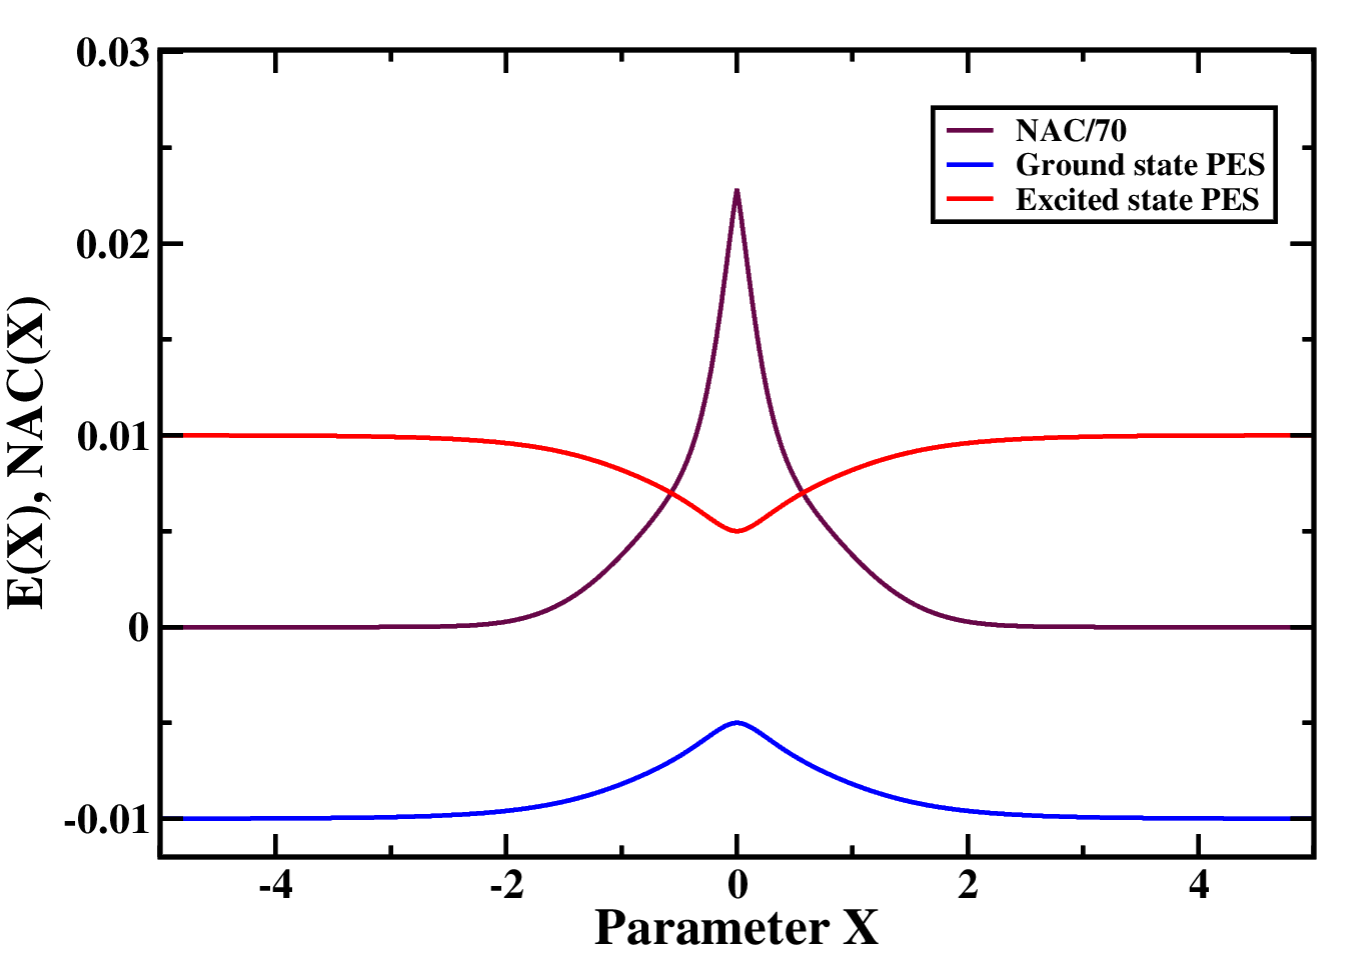
\includegraphics[width = 0.45\textwidth]{images/NAC.png}
        \end{center}
        \caption{Potential energy surfaces and the non-adiabatic coupling for simple avoided crossing}
        \label{fig:PES_Simpleavoided}
    \end{figure}

We also visualize one of the components of non-adiabatic coupling(NAC) vector plotted in \ref{fig:PES_Simpleavoided}. As discussed before, the NAC quantitatively gives us the strength of non-adiabatic transitions. Thus, we expect to see such transitions around $x=0$. Let us use Trajectory Surface Hopping to determine non-adiabatic transition probabilities of the trajectories initiated in asymptotic negative $x$ region of the ground state as a function of its momenta. The probabilities are obtained by keeping track of trajectories. The results are plotted below:
\begin{figure}[H]
\minipage{0.45\textwidth}
  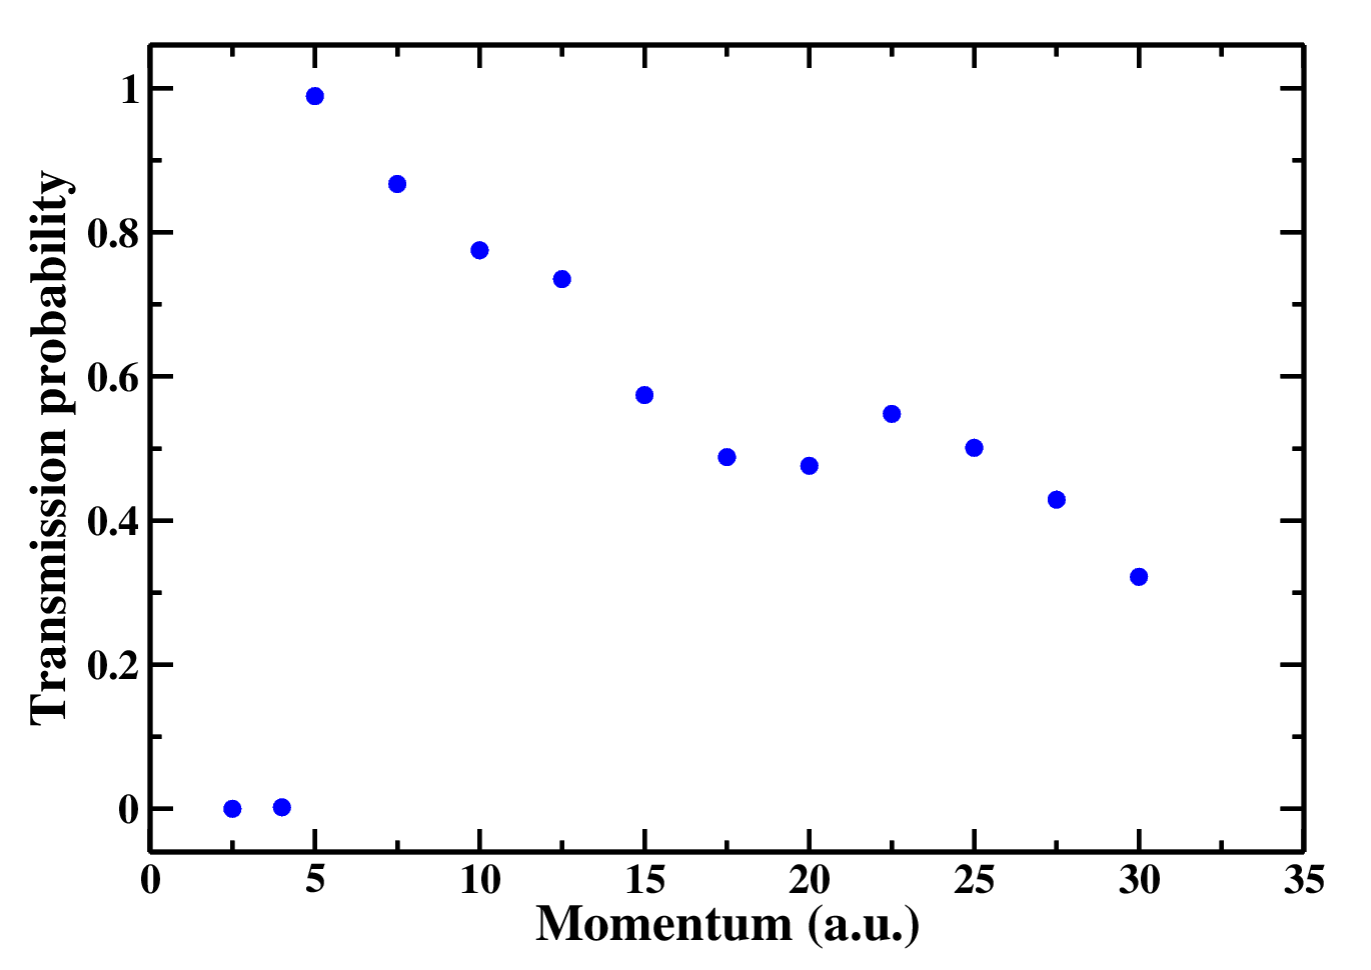
\includegraphics[width=1.1\linewidth]{images/Transmission_prob.png}
  \label{fig:transmission_prob}
  %\caption{A really Awesome Image}\label{fig:awesome_image1}
\endminipage \hspace{1.5em}
\minipage{0.45\textwidth}
  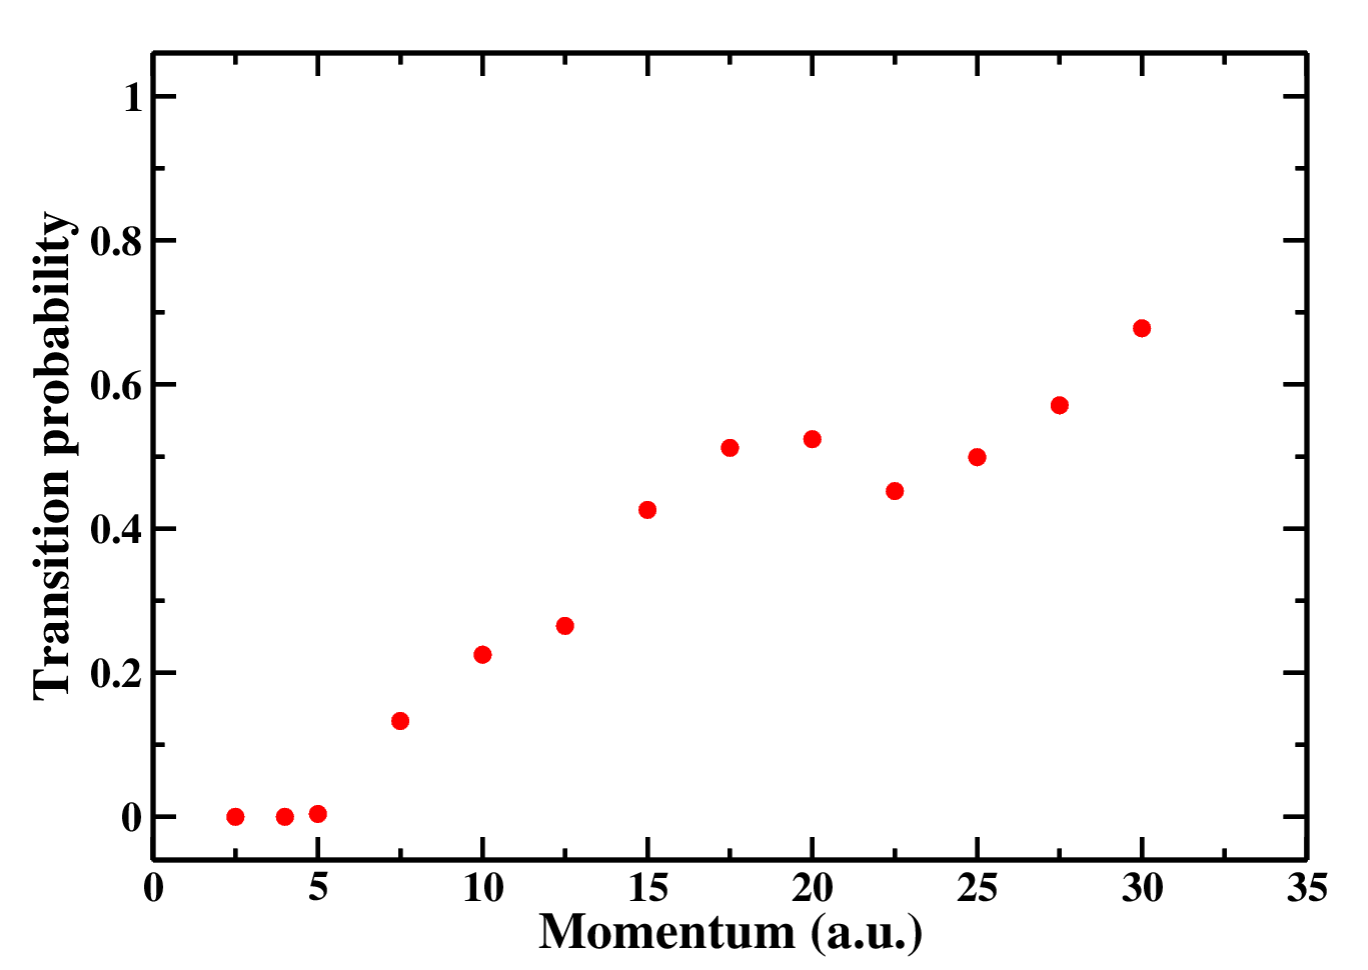
\includegraphics[width=1.1\linewidth]{images/Transition_prob.png}
  \label{fig:transition_prob}
  %\caption{A really Awesome Image}\label{fig:awesome_image2}
\endminipage\hfill
\caption{Transmission probability on the same surface(left) and transition probability(right) as a function of momentum of trajectories}
\label{Transmission and non-adiabatic transition probabilites}
\end{figure}
The most important observation is that we get transitions from the ground state to excited state which is shown in \ref{fig:transition_prob}. We can make an analogy to a diatomic molecule with the parameter $x$ being inter-nuclear distance. This analogy reveals that coupling between nuclear and electronic degrees of freedom can cause atomic transitions to different PES. \\ \\ For low momentum values, the nuclear trajectory cannot overcome the barrier around $x=0$ due to its classical nature in TSH. As its momentum is increased, the probability of transmission across the barrier increases as the energy increases. A further increase in momentum, we see a rise in transition probability and reduce in transmission as expected intuitively. These results are in very good agreement with quantum calculations except a small deviations for low momentum values due to tunnelling.
%\subsection{Extended coupling with Reflection}

\section{Conclusion}

As described above, the trajectory surface hopping simulations capture the non-adiabatic transitions and even agree with quantum calculations well within the statistical error. Also, the conceptual simplicity aids in its popular tool to study non-adiabatic dynamics. However there are certain fundamental problems with TSH. First, the inherent assumption of treating nucleus classically lead to inconsistencies. It cannot describe processes such as nuclear tunneling and dephasing.\cite{curchod,dephasing_1,dephasing_2} Second, surface hopping scheme leads to over-coherences of electronic coefficients over long time which may qualititavely degrade the results.\cite{coherences,wang_TSH} Also, energy should be conserved during the simulation and the velocity is re-adjusted to fulfill this criterion. If the energy conservation cannot be met, a frustrated hop occurs and the standard way is to keep the trajectory unchanged. However, this procedure can lead to a completely different behaviour if a frustrated hop occurs at the crossings. A lot of proposals and work has been done to overcome the shortcomings.\cite{TSH_review,dephasing_2,gen_tsh,quantum_tsh} \\ \\ 
We have successfully written a python wrapper over NWChem platform to simulate non-adiabatic dynamics through TSH. We need to test and benchmark it on different molecular systems. There is a scope for lot of improvement in the code. Our future plans include parallelization of the code to distribute it over nodes. Also, the performance can be improved by replacing the code for crucial parts by a compiled programming language than Python. Apart from performance related issues, the code can be furthered developed to incorporate more functionality to overcome the above problems and also more physics including Spin-Orbit coupling, Floquet formalism for periodic potential, etc.\cite{TSH_review}
    
    \newpage
    \thispagestyle{empty}
    \mbox{}
    \appendix
    \chapter{Proof of Hohenberg-Kohn Theorems}
    \section{Hoheberg-Kohn First theorem}\label{appendix_dft}

\textbf{Theorem Statement:} For any system of interacting particles in an external potential $v_{\text{ext}}(\mathbf{r})$, the density is uniquely determined.(i.e., unique functional of the density)\\ \\ 
\textbf{Proof:} Let there be two different external potentials $v_1(\mathbf{r})$ and $v_2(\mathbf{r})$ that give rise to the same density $n_0(\mathbf{r})$. Therefore, the associated Hamiltonian's $\hat{\mathcal{H}}_1$ and $\hat{\mathcal{H}}_2$ will have different ground state wavefunctions, $\Psi_1$ and $\Psi_2$ that yield the same density $n_0(\mathbf{r})$. According to variational principle, 
\begin{align}
    E_1^0 < \ev**{\hat{\mathcal{H}}_1}{\Psi_2} &= \ev**{\hat{\mathcal{H}}_2}{\Psi_2} + \ev**{\hat{\mathcal{H}}_1 - \hat{\mathcal{H}}_2}{\Psi_2}  \\
    &= E_2^0 + \int d\mathbf{r}[v_1(\mathbf{r})-v_2(\mathbf{r})]n_0(\mathbf{r}) \label{e10}
\end{align}
Similarly,
\begin{align}
    E_2^0 < \ev**{\hat{\mathcal{H}}_2}{\Psi_1} &= \ev**{\hat{\mathcal{H}}_1}{\Psi_1} + \ev**{\hat{\mathcal{H}}_2 - \hat{\mathcal{H}}_1}{\Psi_1}  \\
    &= E_1^0 + \int d\mathbf{r}[v_2(\mathbf{r})-v_1(\mathbf{r})]n_0(\mathbf{r}) \label{e20}
\end{align}
Adding \eqref{e10} and \eqref{e20}
\begin{equation}
    E_1^0 + E_2^0 < E_1^0 + E_2^0 
\end{equation}
which is a contradiction. Hence, the ground state density uniquely determines the external potential. 

\section{Hoheberg-Kohn Second theorem}

\textbf{Theorem Statement:} A universal functional for the energy E[n] can be defined in terms of the density. The exact ground state is the global minimum value of this functional. \\ \\
\textbf{Proof:} According to the first theorem, the density determines the external potential $v_{\text{ext}}(\mathbf{r})$ and hence the wavefunctions making them unique functionals of density. Hence, expectation values of any observables are also unique functionals of density. This allows us to write:
\begin{align}
    E_{v_{\text{ext}}}[n] &= \ev**{\hat{\mathcal{T}} + \hat{\mathcal{V}} + \hat{\mathcal{U}}}{\Psi[n]} \\
    &= \int n(\mathbf{r})v_{\text{ext}}(\mathbf{r}) d\mathbf{r} + F[n]
\end{align}
Clearly this is minimized by the ground state density due to variational principle:
\begin{equation}
    E_1^0 = E[n_0] = \ev**{\hat{\mathcal{T}} + \hat{\mathcal{V}} + \hat{\mathcal{U}}}{\Psi_{\text{gs}}} < \ev**{\hat{\mathcal{T}} + \hat{\mathcal{V}} + \hat{\mathcal{U}}}{\Psi[n]}
\end{equation}

    \chapter{Properties of some Gaussian functions}
    The properties listed here are essential to obtain the recursion relations \eqref{recursive_relations}. The properties listed here are referred from "Gaussian basis sets and molecular integrals", Helgaker Trygve\cite{helgaker}. 
\section{Cartesian Gaussian Functions}\label{appendix_prop}
The Cartesian Gaussian function with origin $\mathbf{A}$ and exponent $\alpha$ is defined as 
\begin{equation}
    G_{ijk}(\mathbf{r},\alpha,\mathbf{A}) = x_A^iy_A^jz_A^k\text{exp}(-\alpha r^2_A)
\end{equation}
where i,j,k are related to angular momentum quantum number as $l = i+j+k$ and $\mathbf{r}_A = \mathbf{r} - \mathbf{A}$. 
\subsection*{Property 1: Factorization}
Cartesian Gaussian can be factorized as follows:
\begin{equation}
    G_{ijk}(\mathbf{r},\alpha,\mathbf{A}) = G_i(x,\alpha,A_x)G_j(y,\alpha,A_y)G_k(z,\alpha,A_z)
\end{equation}
where for example
\begin{equation}\label{x_gaussian}
    G_i(x,\alpha,A_x) = x^i_A\text{exp}(-\alpha x^2_{A_x})
\end{equation}
This property is very helpful in evaluating integrals since it can be factorized into three 1D integrals instead of 3D integral. 
\subsection*{Property 2: Differentiation}
The derivative of Gaussian function \eqref{x_gaussian} with respect to $A_x$ is:
\begin{equation}
    \frac{\partial G_i}{\partial A_x} = -\frac{\partial G_i}{\partial x} = 2\alpha G_{i+1} - iG_{i-1} 
\end{equation}
The derivative depends on the exponent, incremented and a decremented Gaussian. The higher derivatives can also be obtained
\begin{equation}
    \frac{\partial^{q+1} G_i}{\partial A_x^{q+1}} = \left(\frac{\partial}{\partial A_x}\right)^q(2\alpha G_{i+1} - iG_{i-1}) = 2\alpha \frac{\partial^{q} G_{i+1}}{\partial A_x^{q}} - i\frac{\partial^{q} G_{i-1}}{\partial A_x^{q}}
\end{equation}
Defining $\frac{\partial^{q} G_i}{\partial A_x^{q}} \equiv G^q_i$, we get
\begin{equation}
    G_i^{q+1} = 2\alpha G^q_{i+1} - iG^q_{i-1}
\end{equation}
This relation is useful to construct higher derivatives from lower ones.
\subsection*{Property 3: Recurrence}
\begin{equation}
    x_AG_i = G_{i+1}
\end{equation}
\section{Hermite Gaussian Functions}
The Hermite Gaussian centered on $\mathbf{P}$ and exponent $\beta$ is defined as 
\begin{equation}
    \Lambda_{t\mu\nu}(\mathbf{r},\beta,\mathbf{P}) = \left(\frac{\partial}{\partial P_x}\right)^t\left(\frac{\partial}{\partial P_y}\right)^\mu\left(\frac{\partial}{\partial P_z}\right)^\nu
    \text{exp}(-\beta r_P^2)
\end{equation}
with similar interpretations of $t,\mu,\nu$ and $\mathbf{r}_P$.
\subsection*{Property 1: Factorization}
Hermite Gaussian can also be factorized in a similar fashion:
\begin{equation}
    \Lambda_{t\mu\nu}(\mathbf{r},\beta,\mathbf{P}) = \Lambda_t(x,\beta,P_x)\Lambda_\mu(y,\beta,P_y)\Lambda_\nu(z,\beta,P_z)
\end{equation}
where 
\begin{equation}
    \Lambda_t(x,\beta,P_x) = \left(\frac{\partial}{\partial P_x}\right)^t\text{exp}(-\beta x_P^2)
\end{equation}
\subsection*{Property 2: Differentiation}
\begin{equation}
    \frac{\partial\Lambda_t}{\partial P_x} = -\frac{\partial\Lambda_t}{\partial x} = \Lambda_{t+1}
\end{equation}
\subsection*{Property 3: Recurrence}
To find recurrence relation when multiplied by $x_P$, we note:
\begin{equation}
    \Lambda_{t+1} = \left(\frac{\partial}{\partial P_x}\right)^t\frac{\partial\Lambda_0}{\partial P_x} = 2\beta\left(\frac{\partial}{\partial P_x}\right)^tx_P\Lambda_0
\end{equation}
Using the commutator $\left[\left(\frac{\partial}{\partial P_x}\right)^t,x_P\right] = -t\left(\frac{\partial}{\partial P_x}\right)^{t-1}$, we get 
\begin{equation}
    \Lambda_{t+1} = 2\beta(x_p\Lambda_t - t\Lambda_{t-1})
\end{equation}
Rearranging, 
\begin{equation}
    x_p\Lambda_t = \frac{1}{2\beta}\Lambda_{t+1} + t\Lambda_{t-1}
\end{equation}

    \nocite{ulrich,ulrich_1}
    \addcontentsline{toc}{chapter}{Bibliography}
    \printbibliography
    
\end{document}
